% moved in main_(handout/present).tex:
% % \documentclass[en,hyperref=colorlinks]{sdqbeamer}
% % \documentclass[en]{sdqbeamer}
% \mode<presentation> % ??? what is this for?
\graphicspath{ {./img/} {./logos/} } % add further graphics paths here


\usepackage{etex}
\usepackage{graphicx}
\usepackage{color}
\usepackage[export]{adjustbox}
\usepackage{multicol}
\usepackage{pdfpcnotes}
\usepackage{pdfpages}
% \usepackage[dvipsnames]{xcolor}


\usepackage[outputdir={\detokenize{out/main_handout}}]{minted}
\usemintedstyle{pastie}


\usetheme[numbering=counter, progressbar=frametitle, subsectionpage=progressbar]{metropolis}


\date{\today}
% \date{12. Juli 2019}


\institute{Institute for Theoretical Informatics: \newline Artificial Intelligence for Materials Science}
% \titlegraphic{\vspace{4cm} \hspace{7cm} \includegraphics[height=2cm]{Logo_INST}}
\titlegraphic{\vspace{5cm} \hspace{6cm} 
\includegraphics[height=2cm]{AiMat_logo_blue_transparent_rdax_168x76}}

% attempt to reduce space between tableofcontent items in e.g. sectionpage or agenda
\makeatletter
\patchcmd{\beamer@sectionintoc}
  {\vfill}
  {\vskip0\itemsep}
  {}
  {}
\pretocmd{\beamer@sectionintoc}   {\vskip0\itemsep}{}{}
\patchcmd{\beamer@sectionintoc}{\vskip1.5em}{\vskip0.5em}{}{} % <- this one finally works.
\makeatother

% \usepackage{changepage}

% \setbeamertemplate{bibliography item}[text]% {\insertbiblabel}
\addtobeamertemplate{bibliography item}{}{\insertbiblabel}
% \addtobeamertemplate{bibliography item}{\def \bibitemnum {\insertbiblabel}}{}
% \addtobeamertemplate{bibliography entry author}{\insertbiblabel}{}
% \setbeamerfont{bibliography item}{size=\normalsize}
\setbeamercovered{dynamic}

% \AtBeginSection[]
% {
% \begin{frame}[c, plain]
%   \begin{minipage}{22em}
%     \usebeamercolor[fg]{section title}
%     \usebeamerfont{section title}
%
%     % \insertsectionhead\\[-1ex]
%     \iftwocols
%     \begin{multicols}{2}
%     \tableofcontents[currentsection, hideallsubsections]
%     \end{multicols}
%     \else
%     \tableofcontents[currentsection, hideallsubsections]
%     \fi
%
%     % \usebeamertemplate*{progress bar in section page}
%   \end{minipage}
% \end{frame}
% }
% sadly, this does not at all compile and throws weird errors

% from: https://tex.stackexchange.com/questions/365231/enclose-a-custom-quote-environment-in-quotes-from-csquotes
\usepackage[style=british]{csquotes}

\def\signed #1{{\leavevmode\unskip\nobreak\hfil\penalty50\hskip1em
  \hbox{}\nobreak\hfill #1%
  \parfillskip=0pt \finalhyphendemerits=0 \endgraf}}

\newsavebox\mybox
\newenvironment{aquote}[1]
  {\savebox\mybox{#1}\begin{quote}\openautoquote\hspace*{-.7ex}}
  {\unskip\closeautoquote\vspace*{1mm}\signed{\usebox\mybox}\end{quote}}


\iftwocols
\AtBeginSection[]
{
\begin{frame}[c, plain]
  \begin{minipage}{22em}
    \usebeamercolor[fg]{section title}
    \usebeamerfont{section title}
    % \insertsectionhead\\[-1ex]
    % \usebeamertemplate*{progress bar in section page} % progress bar
    \begin{multicols}{2}
    \tableofcontents[currentsection, hideallsubsections]
    \end{multicols}
  \end{minipage}
\end{frame}
}
\else

\AtBeginSection[]
{
\begin{frame}[c, plain]
  \begin{minipage}{22em}
    \usebeamercolor[fg]{section title}
    \usebeamerfont{section title}
    % \insertsectionhead\\[-1ex]
    \tableofcontents[currentsection, hideallsubsections]
    % \usebeamertemplate*{progress bar in section page}
  \end{minipage}
\end{frame}
}
\fi

\AtBeginSubsection[]
{
\begin{frame}[c,plain]
  \begin{minipage}{22em}
    \raggedright
    \usebeamercolor[fg]{section title}
    \usebeamerfont{section title}
    \insertsectionhead\\[-1ex]

    \usebeamertemplate*{progress bar in section page}
    \par
    \ifx\insertsubsectionhead\@empty\else%
      \usebeamercolor[fg]{subsection title}%
      \usebeamerfont{subsection title}%
      \vspace{0.5cm}
      \tableofcontents[sectionstyle=hide/hide,subsectionstyle=show/shaded/hide]
    \fi
  \end{minipage}
\end{frame}
}


%%%%%%%%%%%%%%%%%%%%%%%%%%%%%%%%%%%%%%%%%%%%%%%%%%%%%%%%%%%%%%%%%%%%%%%%%%%%%%%%%%%%%%%%%%%%%%%%%%%
% Newcommand definitions
% - code[1]
% - backupbegin
% - backupend
% - mailto[1]
% - todo[1]
% Environments:
% - codeboxed[1]


\newcommand{\code}[1]{
    \begin{center}
    \setlength{\fboxrule}{1pt}
    \setlength{\fboxsep}{8pt}
        {\fbox{\parbox{0.81\textwidth}{#1}}}
   \end{center}
}

\newenvironment{codeboxed}[1]
        {\begin{minipage}{\linewidth}\begin{center}#1\\[1ex]\begin{tabular}{|p{\textwidth}|}\hline}
        {\\\hline\end{tabular}\end{center}\end{minipage}}


\newcommand{\backupbegin}{
   \newcounter{finalframe}
   \setcounter{finalframe}{\value{framenumber}}
}

\newcommand{\backupend}{
   \setcounter{framenumber}{\value{finalframe}}
}


\newcommand{\mailto}[1]{
    \href{mailto:#1}{#1}
}

\newcommand{\todo}[1]{
    {\Large\color{red}{(TODO: #1)}}
}

% \definecolor{green1}{RGB}{38, 69, 37} % #264525
\definecolor{green1}{RGB}{72, 129, 69} % #488145
% \definecolor{blue1}{RGB}{7, 43, 94} % #072b5e
\definecolor{blue1}{RGB}{14, 82, 179} % #0e52b3
% \definecolor{violet1}{RGB}{58, 38, 68} % #3a2644
\definecolor{violet1}{RGB}{108, 72, 126} % #6c487e
% \definecolor{orang1}{RGB}{, , 0} % #663400
\definecolor{orang1}{RGB}{193, 98, 0} % #c16200

\newcommand{\gray}[1]{
    \textcolor[gray]{0.65}{#1}
}

\newcommand{\green}[1]{
    \textcolor{green1}{#1}
}
\newcommand{\blue}[1]{
    \textcolor{blue1}{#1}
}
\newcommand{\vio}[1]{
    \textcolor{violet1}{#1}
}
\newcommand{\orang}[1]{
    \textcolor{orang1}{#1}
}



%%%%%%%%%%%%%%%%%%%%%%%%%%%%%%%%%%%%%%%%%%%%%%%%%%%%%%%%%%%%%%%%%%%%%%%%%%%%%%%%%%%%%%%%%%%%%%%%%%%
% begin document

\begin{document}
\addtocounter{framenumber}{1}
\maketitle


%%%%%%%%%%%%%%%%%%%%%%%%%%%%%%%%%%%%%%%%%%%%%%%%%%%%%%%%%%%%%%%%%%%%%%%%%%%%%%%%%%%%%%%%%%%%%%%%%%%
% Agenda

\iftwocols

\begin{frame}[c,plain]% {Agenda}
    \begin{minipage}{22em}
    \usebeamerfont{section title}
    \usebeamercolor[fg]{section title}
    % \usebeamertemplate*{progress bar in section page} % progress bar
    \begin{multicols}{2}
    \tableofcontents[hideallsubsections]
%   \tableofcontents[]
    \end{multicols}
    \end{minipage}
\end{frame}

\else

\begin{frame}[c,plain]% {Agenda}
    \begin{minipage}{22em}
    \usebeamerfont{section title}
    \usebeamercolor[fg]{section title}
    \tableofcontents[hideallsubsections]
%   \tableofcontents[]
    \end{minipage}
\end{frame}
\fi



% TODO: convert all \pnote to english. Why did I not do that before

% \section{Motivation}
% \begin{frame}[c]{The Need for 3D Deep Learning}
%     \large
%     \begin{figure}
    \captionsetup[subfigure]{labelformat=empty}
    \begin{subfigure}{0.3\textwidth}
        % lidar car visualization
        Robot Perception \\
        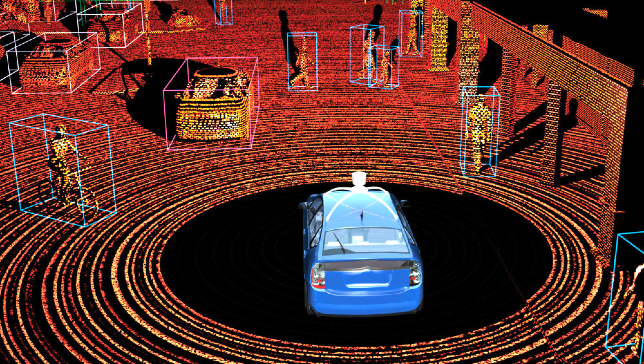
\includegraphics[height=0.35\textheight]{p02_6}
        \caption{source: Scott J Grunewald}
    \end{subfigure}
    \hspace{5mm}
    \begin{subfigure}{0.3\textwidth}
        % phone AR
        Augmented Reality \\
        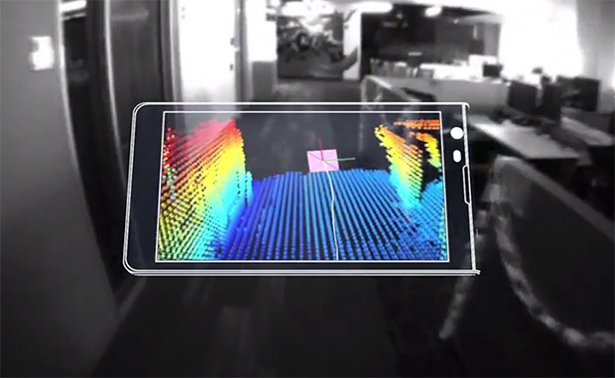
\includegraphics[height=0.35\textheight]{p02_8}
        \caption{source: Google Tango}
    \end{subfigure}
    \hspace{2mm}
    \begin{subfigure}{0.3\textwidth}
        % solidworks 3D objects
        Shape Design \\
        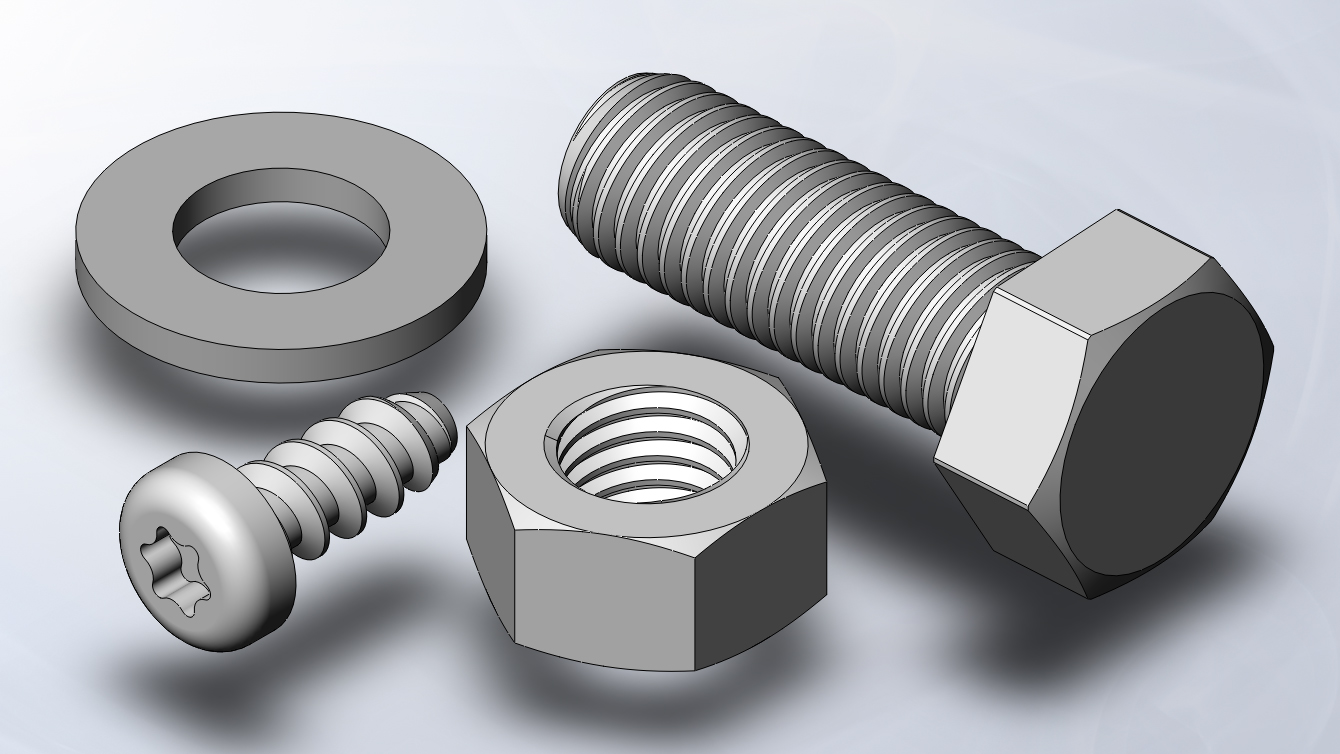
\includegraphics[height=0.35\textheight]{p02_7}
        \caption{source: solidworks}
    \end{subfigure}
    \blfootnote{Figures and captions from CVPR presentation to \cite{qi2017pointnet}.}
\end{figure}

%     \Large
%     \vspace{1em}
%     A number of emerging 3D applications shape the need for 3D deep learning.
%     \pnote{
%         Es entstehen viele Anwendungen die Wahrnehmung  \\
%         oder Interaktion in 3D benötigen.
%         \par
%         - viele Anwendungen im 3D bereich entstehen \\
%         - brauchen Wahrnehmung oder Interaktion in 3D \\
%         - um diese zu bedienen: hoher bedarf \\
%         - spezifisch auf 3D zugeschnitten \\
%         - Erster: PointNet \\
%     }
% \end{frame}


\section{Representation}
\begin{frame}[c]{Common Representations of 3D Data}
    \begin{figure}
    % \captionsetup[subfigure]{labelformat=empty, size=\large, labelfont={black, bf}}
    \captionsetup[subfigure]{labelformat=empty, font={large, color=black}}
    \begin{subfigure}{0.23\textwidth}
        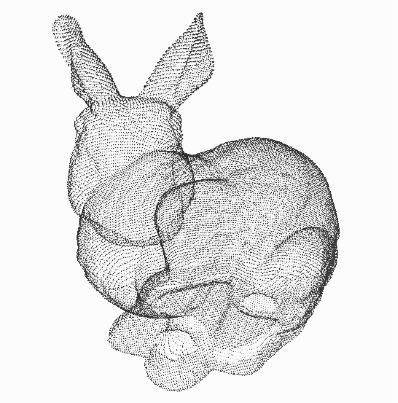
\includegraphics[height=0.35\textheight]{p04_12}
        \caption{Point Cloud}
    \end{subfigure}
    \begin{subfigure}{0.23\textwidth}
        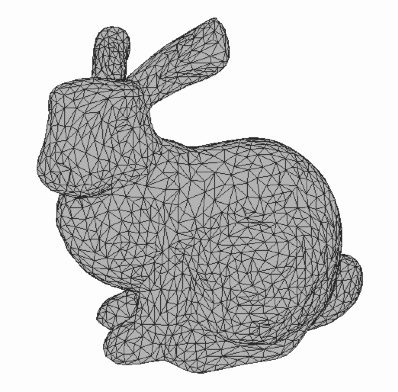
\includegraphics[height=0.35\textheight]{p04_13}
        \caption{Mesh}
    \end{subfigure}
    \begin{subfigure}{0.23\textwidth}
        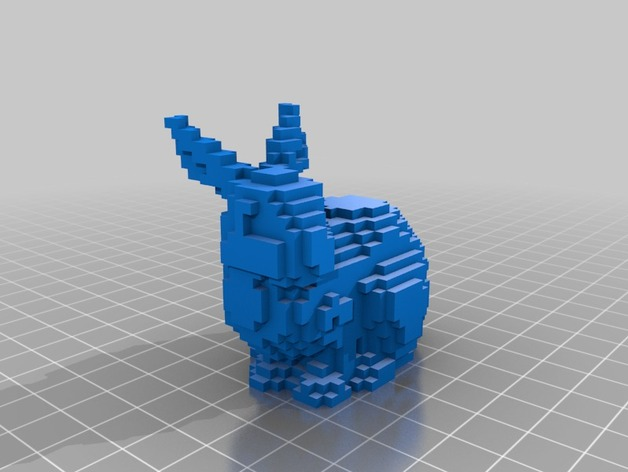
\includegraphics[height=0.35\textheight]{p04_14}
        \caption{Volumetric}
    \end{subfigure}
    \hspace{1mm}
    \begin{subfigure}{0.23\textwidth}
        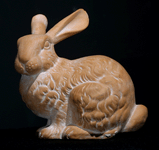
\includegraphics[height=0.35\textheight]{p04_15}
        \caption{View Rendering}
    \end{subfigure}
    \blfootnote{Figures and captions (partially) from CVPR presentation to \cite{qi2017pointnet}.}
\end{figure}

    \Large
    \vspace{1em}
    Contrary to 2D, 3D has many different popular representations.
    \pnote{Auszug an Beispielen}
\end{frame}


\begin{frame}[c]{Canonical Representation: Point Cloud}
    \large
    \begin{columns}
        \column{0.32\textwidth}
        \begin{itemize}
            \item Point cloud is close to \textbf{raw depth sensor data}
            \item Point cloud is \textbf{canonical} (easy conversion from and to other representations)
        \end{itemize}
        \color{ocre}
        \normalsize
        \vspace{2em}
        Individual figures from CVPR presentation to \cite{qi2017pointnet}
        \column{0.68\textwidth}
        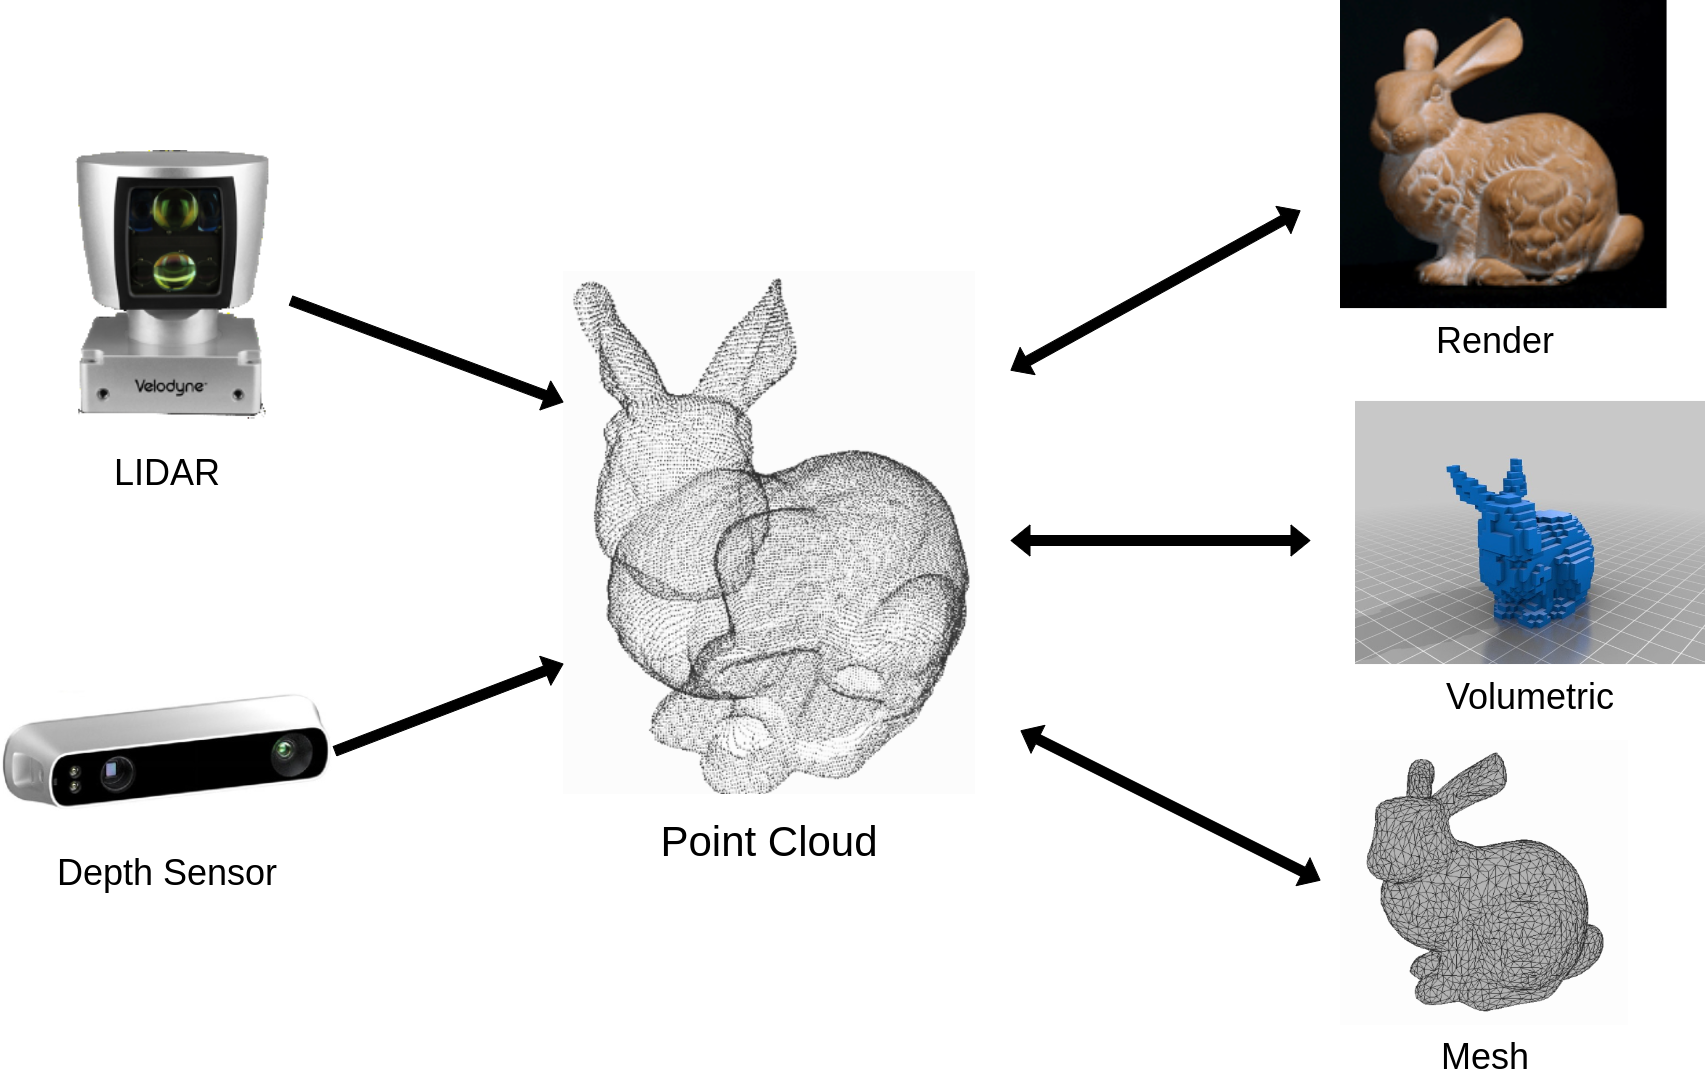
\includegraphics[height=0.75\textheight]{canonical}
    \end{columns}
    \pnote{
        - Am nächsten zu ursprünglichen Tiefendaten\\
        - Kanonische Form: andere lassen sich einfach umwandeln \\
        Allerdings: wenig Arbeit zu Point Cloud Features
    }
\end{frame}

 % done
\section{Related Work}
\begin{frame}[c]{Point Cloud Features}
    \large
    \begin{figure}
        \captionsetup[figure]{labelformat=empty}
        % \captionsetup[subfigure]{labelformat=empty}
        \small
        \section{Project Results}

% \subsection{Upgrade Dependencies}
% 
% \begin{frame}[c]
%     From Django 2 to Django 3 \\
%     (Django 4 released during the project, has been decided to go to 3 in production first) \\
%     Now requires \mintinline{python}{DEFAULT_AUTO_FIELD = "django.db.models.AutoField"}
% \end{frame}

\subsection{Proper Logging}

\begin{frame}[c]{Changes to Logging}
    \large
    \begin{itemize}[<+(1)->]
        \item Logging used to be over individual `print` statements
        \item Properly defined Logging levels (debug, info, warn, error, critical)
        \item Logging to console, syslog and file
        \item Differing formatter for console and other (timestamps, ...)
        \item Rotating files: Keep last five days, overwrite after
    \end{itemize}
\end{frame}

\begin{frame}[c]{Logging Before: Example} 
    \todo{Screenshot: Logging before, Optional}
\end{frame}

\pic{Logging Now: Example}{33}

\subsection{Automatically generate Documentation}

\begin{frame}[c]{Why is this worth trying?} 
    \begin{itemize}[<+(1)->]
        \item 
    \end{itemize}
\end{frame}

\begin{frame}[c]{Automatically Generate Documentation}
    \begin{multicols}{2}
        \large
        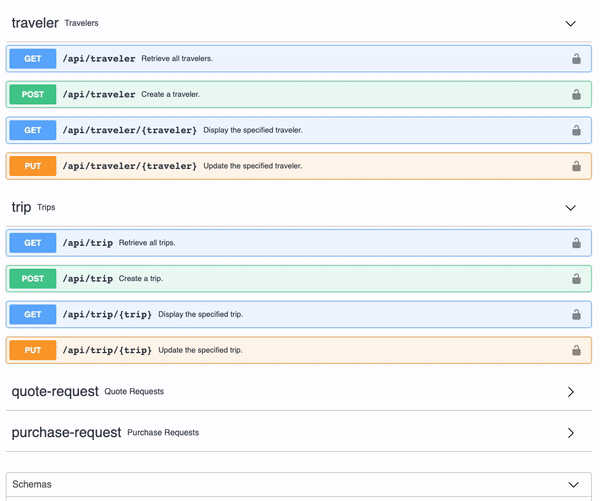
\includegraphics[width=0.5\textwidth]{swagger} \\
        (Example) \\
        Failed, because:
        \begin{itemize}[<+(1)->]
            \item Mainly used to generate documentation for JSON endpoints
            % \item Few comments to generate documentation from
            \item 'Primitive' Views lacking important information for automatic generation
        \end{itemize}
        Was worth a try.
    \end{multicols}
\end{frame}

\subsection{What Research is the Storage used for?}

\begin{frame}[c]{What Research is the Storage used for?}
    \begin{multicols}{2}
    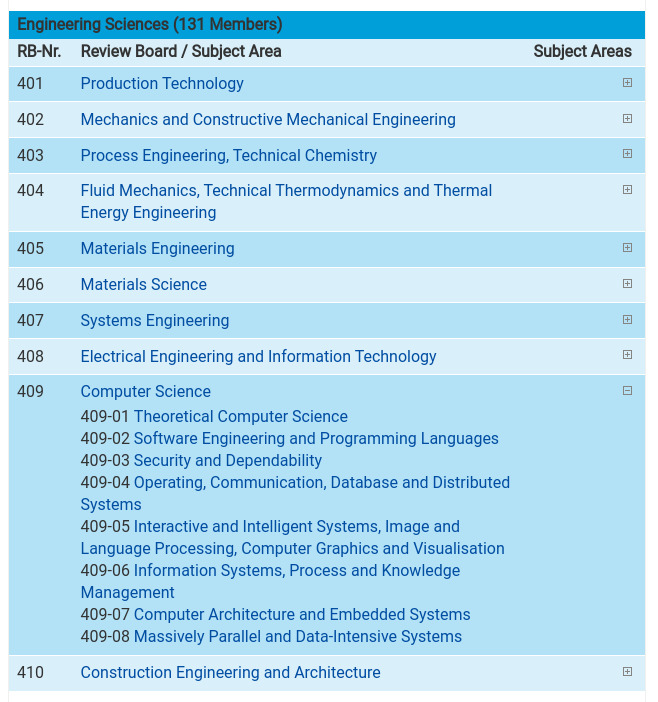
\includegraphics[width=0.5\textwidth]{Selection_032}
    \large
        \begin{itemize}[<+(1)->]
            \item We want to know more about our users
            \item This includes affiliation of research projects
            \item Good separation in subject areas from 'Deutsche Forschungsgesellschaft'
        \end{itemize}
    \end{multicols}
\end{frame}

\pic{Selection of DFG Subject Area upon Project Creation}{10}

\begin{frame}[c]{Selection of DFG Discipline}
    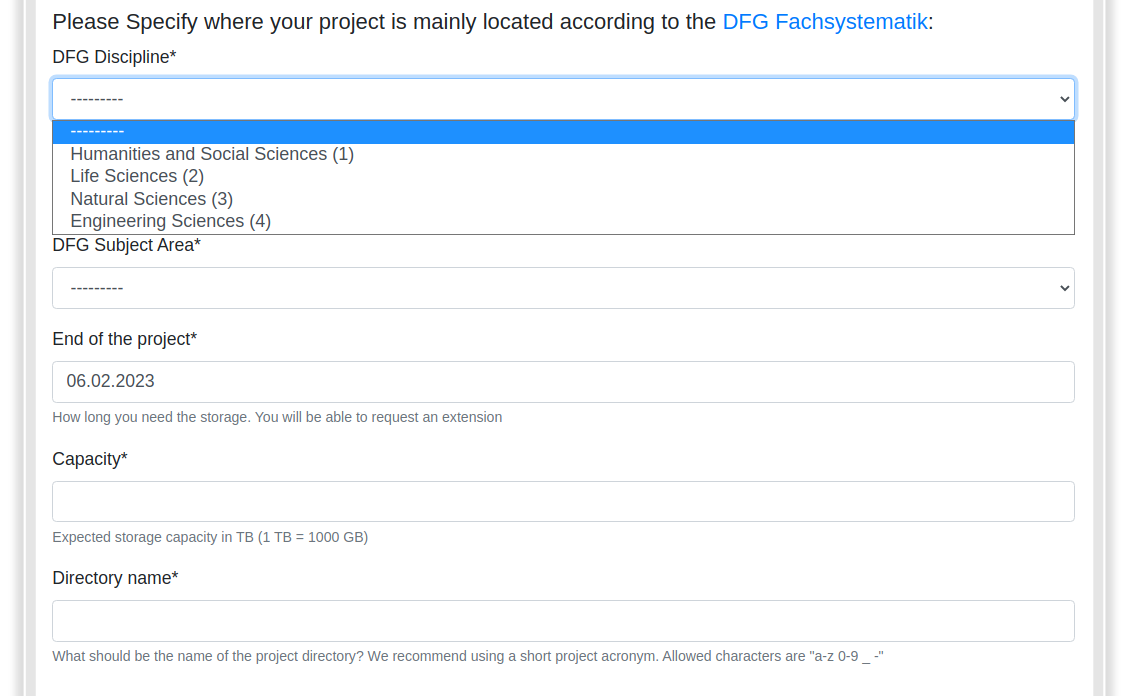
\includegraphics[width=\textwidth]{select_discipline}
\end{frame}
\begin{frame}[c]{Selection of DFG Subject without Board}
    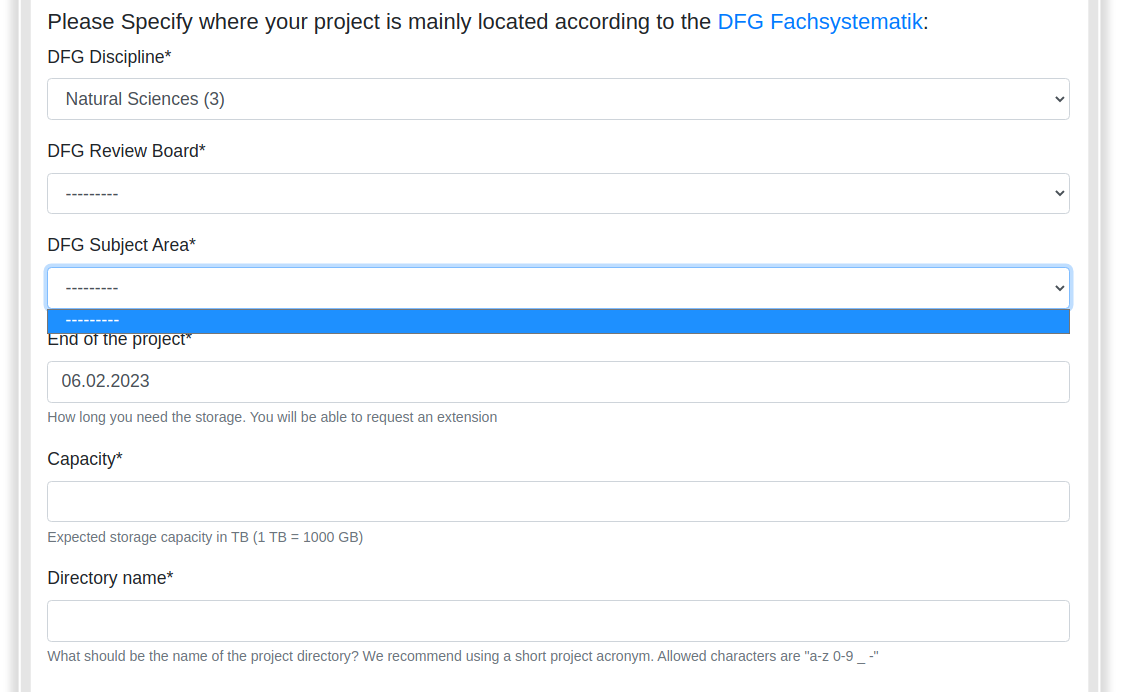
\includegraphics[width=\textwidth]{select_subject1}
\end{frame}
\begin{frame}[c]{Selection of DFG Subject}
    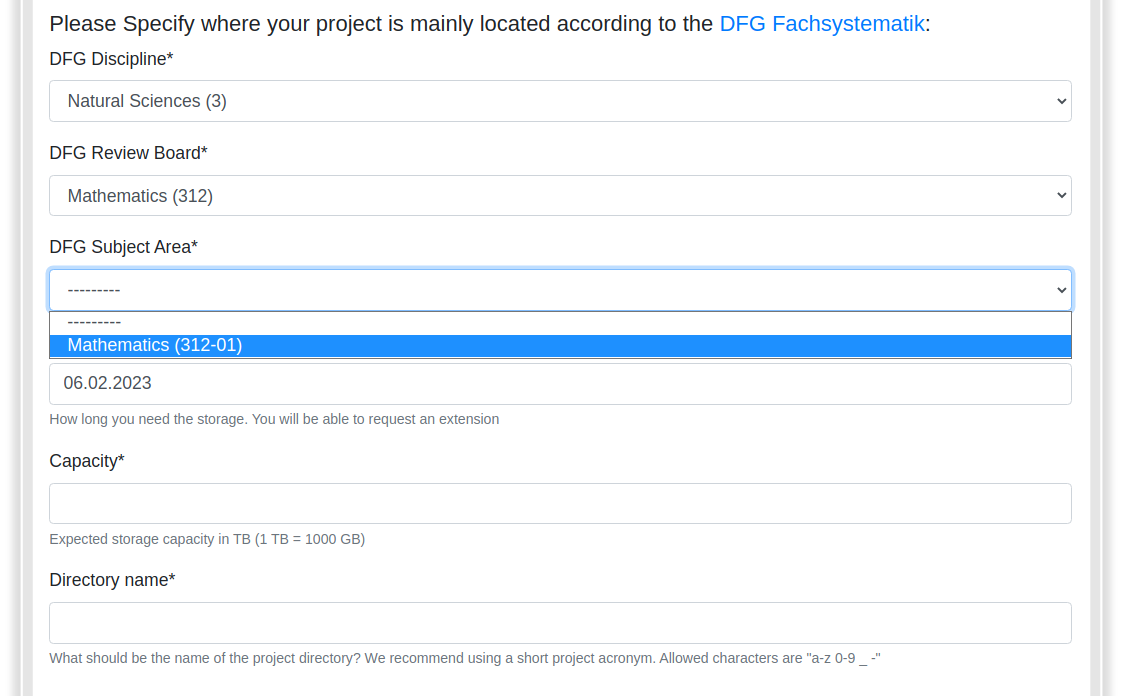
\includegraphics[width=\textwidth]{select_subject2}
\end{frame}


\begin{frame}[c,fragile]{Code Requesting Fields for Boards}
    \footnotesize
    \inputminted[linenos=true]{javascript}{code/board_request.js}
\end{frame}


\begin{frame}[c,fragile]{Backend answering with available Fields}
\footnotesize
    \begin{minted}[linenos]{python}
## urls.py
path('ajax/fields/', views.view_science_fields, name="ajax_load_fields"),

## views.py
def view_science_fields(request):
    b_pk = request.GET.get('board')  # we get the pk of the selected board
    if b_pk:  # select available Fields from this Board
        fields = Science_Field.objects.filter(board__pk=b_pk) 
        return render(request, 'dropdown_list_options.html',
                      {'options': fields})
    return render(request, 'dropdown_list_options.html',
                  {'options': Science_Field.objects.none()})
\end{minted}
\end{frame}

\subsection{Diff csv to DFG schema in database}

\begin{frame}[c]{The DFG schema changes frequently}
    \large
    \begin{itemize}[<+(1)->]
        \item The DFG schema changes every four years
        \item It was last changed in 2020
        \item So it'll change again in two years
        \item Not clear how much (probably not a whole lot)
    \end{itemize}
    \pause
    So I implemented a command to compare any csv to what is currently in the
    database: \mintinline{bash}{manage.py dfg_schema_diff}
\end{frame}


% \begin{frame}[fragile]{Usage of \texttt{dfg_schema_diff}}
\begin{frame}[fragile]{Usage of \texttt{dfg\_schema\_diff}}
    \scriptsize
\begin{verbatim}
usage: manage.py dfg_schema_diff [-h] [--locale LOCALE] [--columns COLUMNS]
                     ...
                     FILE

Show difference from given file schema to DFG schema in database. By default,
ignores the now deprecated hierarchy level 1. ...

positional arguments:
  FILE                  Path to dfg_systematic.csv

options:
  -h, --help            show this help message and exit
  --locale LOCALE       Set the language of the name column to select. Can correctly select
                        both '<locale>' and 'prefLabel@<locale>' columns. (Default: 'en')
  --columns COLUMNS     Dictionary mapping columns (numbers) to expected values "level" (in
                        the hierarchy, category: 0, deprecated/ignored: 1, board: 2, field:
                        3), "notation" (e.g. 101-27), and locale translations, e.g. "en"
                        (double quotes are important!). Defaults to auto.
  ...                   ...
\end{verbatim}
\end{frame}

% \subsection{Rename Models}
% 
% \begin{frame}[c]
%     % Order -> LSDFProject
%     % PersonOrder -> ProjectRole
%     % ...
%     Worked quite well, generated some migrations
% \end{frame}

% \subsection{Attempt to rename entire App}
% 
% \begin{frame}[c]
%     Failed, ultimately unclear why, requires deep django/database knowledge.
% \end{frame}


\subsection{Attempt to properly modularize PersonForm}

\begin{frame}[c]
    Explain the problem (show exemplary code) of redundancy
    Managed to get quite far, very good (deep) learning example, and absolutely
    possible. just requires some more time than expected.
    Nags me that it's not modular yet. Some day.
\end{frame}


\subsection{Extension Requests}

\begin{frame}[c]
    WHY Extension Requests
\end{frame}

\begin{frame}[c]{Extension Requests}
    Much-requested feature.
    \todo{Overview of newly introduced routes, views, forms, models and relations}
\end{frame}

        \caption{Overview from \url{https://github.com/PointCloudLibrary/pcl/wiki/Overview-and-Comparison-of-Features}}
    \end{figure}
    Most existing point cloud features are \textbf{handcrafted for specific tasks}. \\
    \pnote{
        Die meisten zuvor existierenden Features sind \\
        nur für bestimmte Aufgaben. \\
        Skaliert sehr schlecht für neue Aufgaben.
        \par
        Die Tabelle listet ein paar davon.
    }
\end{frame}


\begin{frame}[c]{Conversion to Other Representations}
    \begin{columns}
        \column{0.1\textwidth}
        \column{0.6\textwidth}
        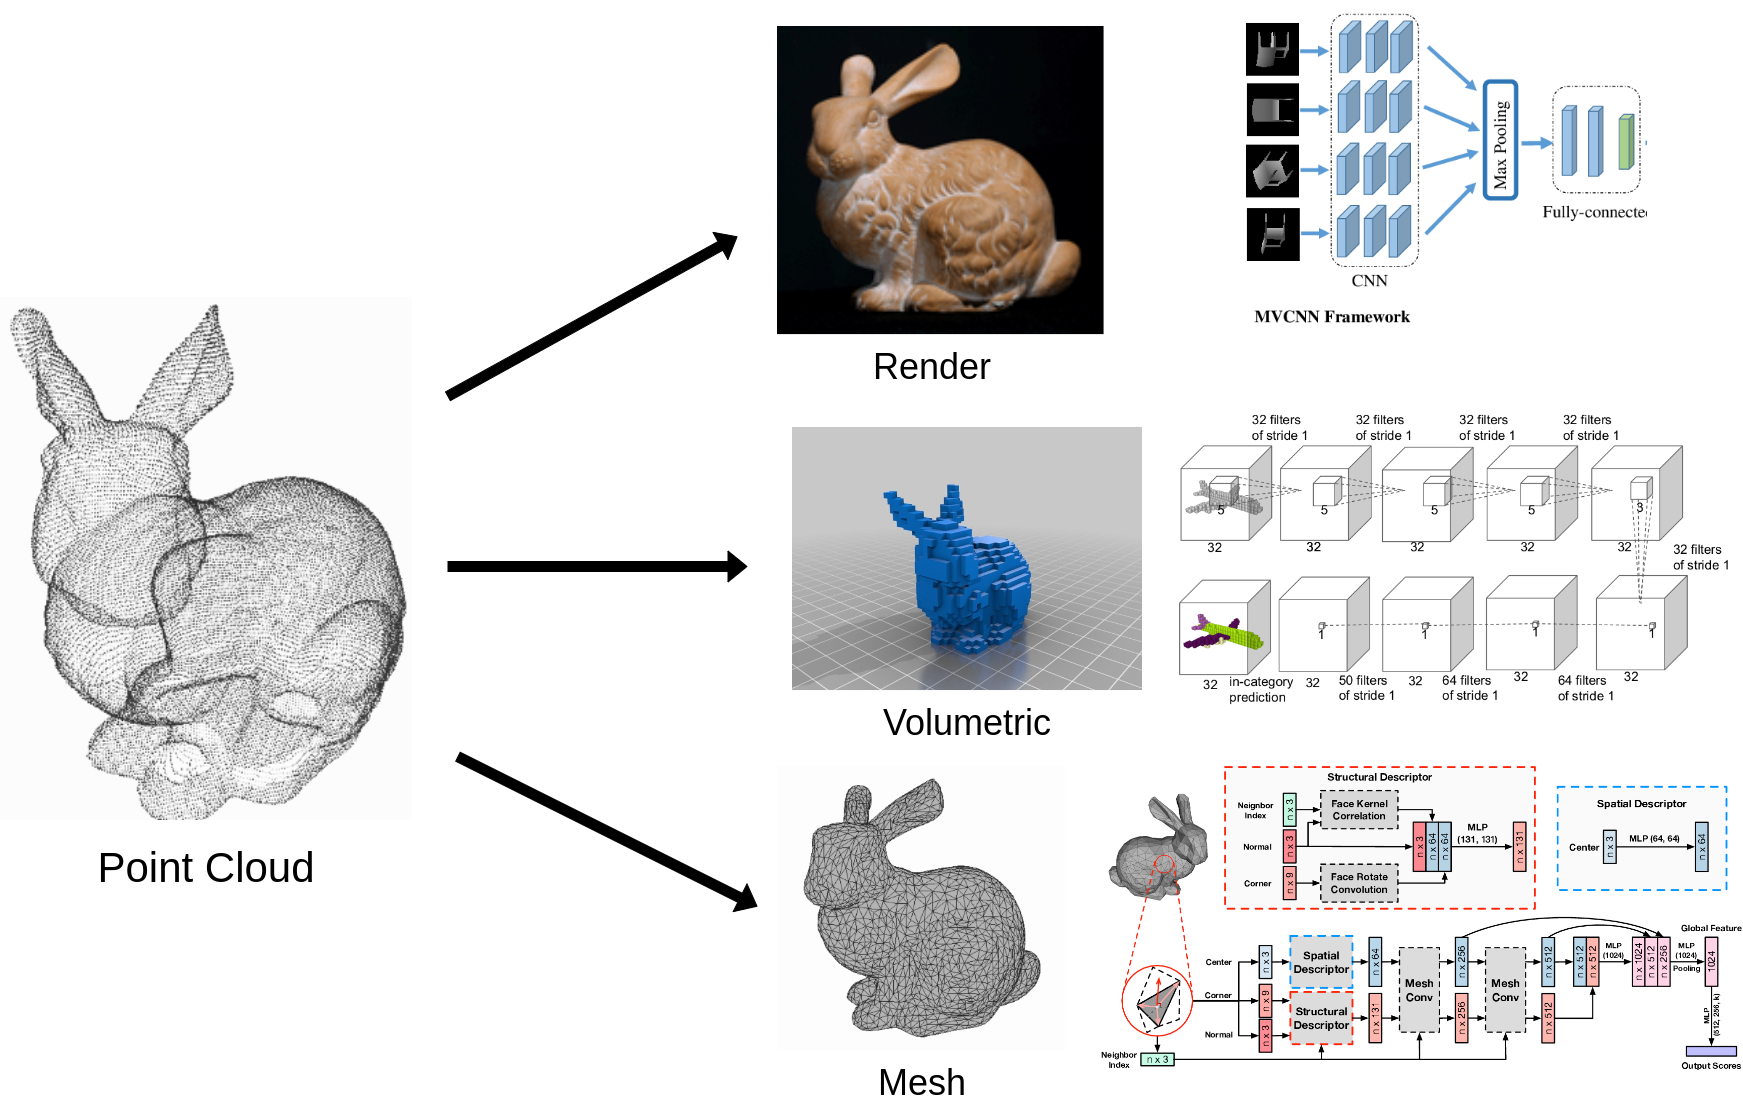
\includegraphics[height=0.75\textheight]{conversion}
        \column{0.3\textwidth}
        \color{ocre}
        Figures from:
        \begin{itemize}
                \color{ocre}
            \item Bunnies: CVPR presentation to \cite{qi2017pointnet} \\
            \item MVCNN: \cite{li2019angular} \\
                % \item 3D-CNN-image: \cite{roy2019ecnn} \\
            \item 3D-CNN: Supplemental to \cite{qi2017pointnet} \\
            \item Mesh-Net: \cite{feng2019meshnet} \\
        \end{itemize}
    \end{columns}
    \pnote{
        Es gibt bereits Arbeiten auf Point Cloud. \\
        \par
        Allerdings wandeln diese Punktwolken erst \\
        in andere Darstellungen um, und verwenden \\
        anschließend bereits existierende Architekturen.
    }
\end{frame}


% \begin{frame}[c]{Learning on Unordered Sets}
%
%     A point cloud is an unordered set of vectors from the data structure point of
%     view. Most works in deep learning however look at regular input structures like
%     ordered sequences of images, volumes or points. Unordered point clouds are
%     rarely considered. One recent work \cite{vinyals2015order} attempts to impose
%     order on unordered input sets via the attention mechanism. This work focuses on
%     generic sets and NLP applications, which lacks the characteristics of geometry
%     in the sets.
%
%     \todo{Order Matters! Find Visualization .... none in paper}
%
%     \todo{alternatively, exclude from presentation}
% \end{frame}


\begin{frame}[c]
    \LARGE
    \begin{centering}
        Research Question: \\
        \vspace{1cm}
        Can we achieve effective \textbf{feature learning directly} on point clouds?
    \end{centering}
    \pnote{
        Frage: Können wir Feature Learning \\
        direkt auf Punktwolken erreichen? \\
        \par
        Die Antwort ist ja.
    }
\end{frame}

    % done
\section{PointNet}

\begin{frame}[c]{Introduction to PointNet}
    \large
    \begin{multicols}{2}
        \begin{itemize}
            \item End-to-end learning for unordered point cloud data
            \item Unified framework for previously seperate and specialized tasks
                \begin{itemize}
                    \item Object Classification
                    \item Object Part Segmentation
                    \item Semantic Scene parsing
                \end{itemize}
        \end{itemize}
        \begin{figure}
            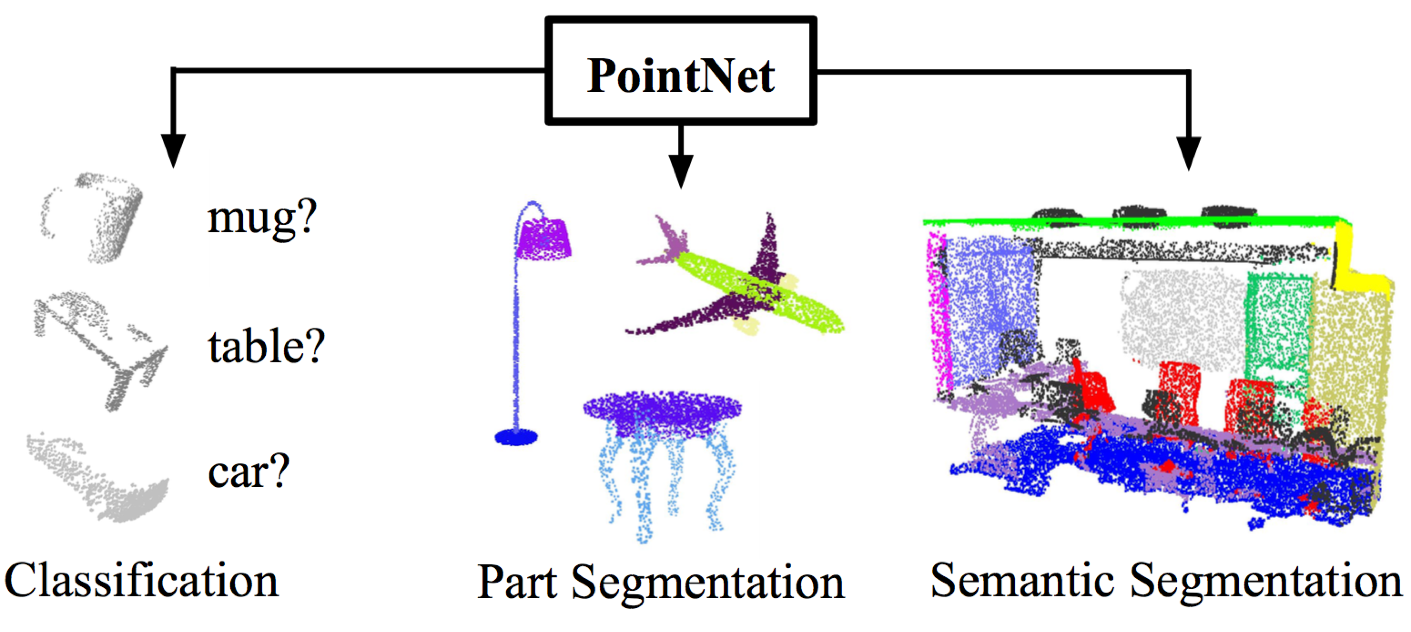
\includegraphics[width=0.5\textwidth]{p12_29}
            \caption{Figure from \cite{qi2017pointnet}.}
        \end{figure}
    \end{multicols}
    \pnote{
        Ergebnis davon: PointNet, einheitliche \\
        architektur für verschiedene Aufgaben
        \par
        Ende-zu-Ende lernen für Punktwolken \\
        Vereinheitlichen von zuvor spezialisierten Aufgaben
    }
\end{frame}


\begin{frame}[c]{Challenges}
    \Large
    \begin{multicols}{2}
        \begin{itemize}[<+->]
            \item Unordered point sets as input
                \begin{itemize}[<1->]
                    \item Model needs to be invariant to $N!$ permutations
                \end{itemize}
            \item Invariance under geometric transformations
                \begin{itemize}[<2->]
                    \item Geometric transformations applied to point cloud data
                        should not alter classification results
                \end{itemize}
        \end{itemize}
        \centering
        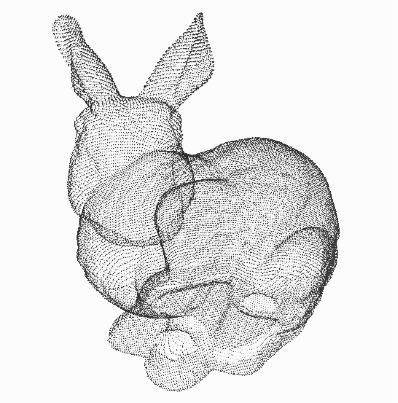
\includegraphics[height=0.35\textheight]{p04_12}
        \includegraphics<2->[height=0.35\textheight]{geometric_transformations}
    \end{multicols}
    \blfootnote{Point cloud figure from CVPR presentation to \cite{qi2017pointnet}.}
    \blfootnote{Geometric transformation figure from \cite{BibEntry2019Oct}.}
    \pnote{
        Herausforderung: Umgang mit Punktwolken. Muss: \\
        - Unsortierte Mengen als eingabe \\
        - Keine Kanonische Höherdimensionale Sortierung \\
        - Invarianz über Geometrische Transformationen
    }
\end{frame}
 % done
\section{Unordered Input}
\begin{frame}[c]{Unordered Point Sets}
    \large
    \begin{multicols}{2}
        A set of points $p_i := (x_i, y_i, z_i)$
        $$ \{ p_1, p_2, \ldots, p_n\} $$
        \vspace{1em}
        might be represented by any of its vector permutations $ [ p_{\pi_1}, p_{\pi_2}, \ldots, p_{\pi_n} ] $ for any permutation $\pi$. \\
        \vspace{1em}
        Since point cloud data is \underline{orderless}, it requires
        invariance over input permutations when consumed directly.
        \vspace{2em}
        \begin{figure}
            \centering
            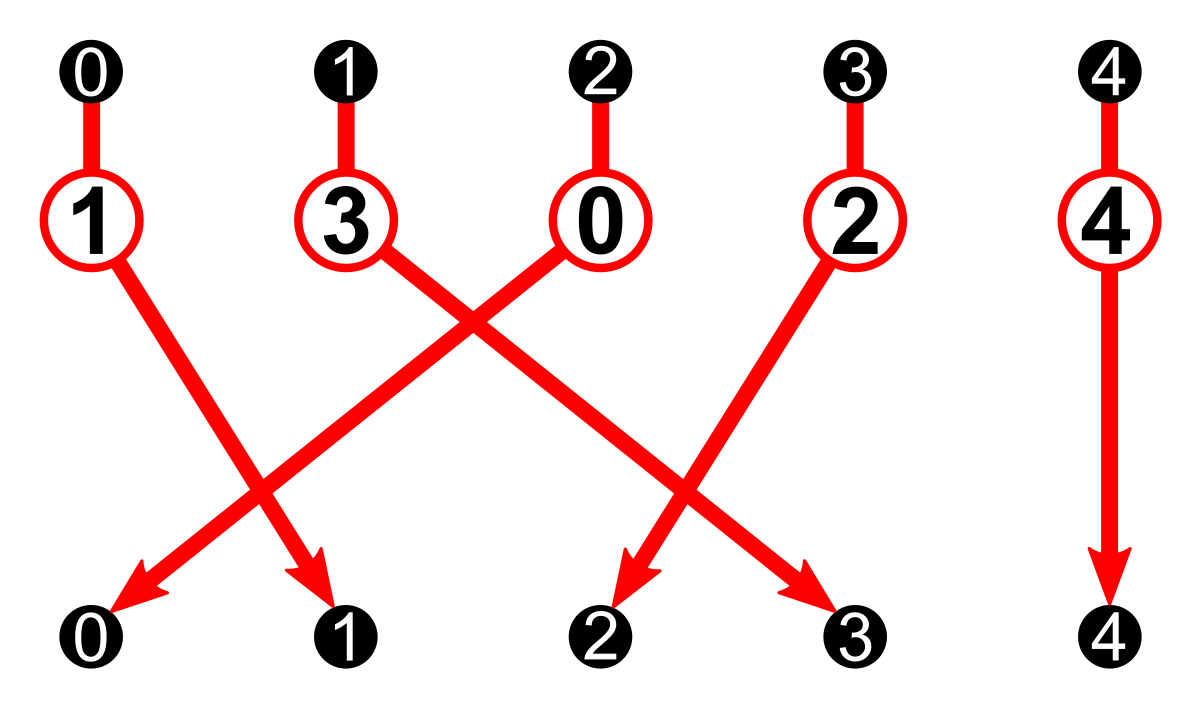
\includegraphics[height=0.4\textheight]{permutation}
            \caption{\textbf{Example Permutation.} \\Figure under CC-BY-SA 4.0 from \cite{BibEntry2022Jun2}}
        \end{figure}
    \end{multicols}
    \pnote{
        Erste Herausforderung: \\
        - umgehen mit beliebigen Eingabe-permutation \\
        - wir verwenden Vektoren um Eingaben darzustellen \\
        - können auch weitere Dimensionen haben \\
        - keine stabile Sortierung der Punkte möglich \\
        - !tricks: neu Messen, anderes Datenset, anderer Sensor \\
        - Mathematisch: tricksen nicht Möglich
    }
\end{frame}


\begin{frame}[c]{Solution: Symmetric Functions}
    \large
    Symmetric functions are invariant over argument permutations $\pi$:
    $$ f(x_1, x_2, \ldots, x_n) \equiv f(x_{\pi_{1}}, x_{\pi_{2}}, \ldots, x_{\pi_{n}}) $$

    \pause

    Examples for symmetric functions:

    \begin{itemize}
        \item $\max$
        \item sum / addition
        \item mean
    \end{itemize}
    \vspace{1em}

    Q: How to integrate a symmetric function into a neural network architecture?
    \pnote{
        Mathematisch: neuronales Netz nur eine Funktion \\
        Funktional betrachtet: Symmetriedarstellung über fkt \\
        \par
        Symmetrisch, wenn Funktionswert bei Argumentenvertausch \\
        gleich bleibt.
        \par
        Es gibt viele Symmetrische Funktionen. Beispiele
        \par
        Frage wird: Wie können eine Symmetrische Funktion in \\
        Architektur von Neuronalem Netz integrieren?
    }
\end{frame}


\begin{frame}[c]{One Symmetric Function is All You Need}
    \large
    A concatenation of functions ($\gamma \circ g(h,..)$) is symmetric if the central function $g$ is symmetric:
    $$ f(x_1, x_2, \ldots, x_n) = \gamma \circ g(h(x_1), \ldots, h(x_n)) $$
    \pause
    \centering
    \begin{figure}
        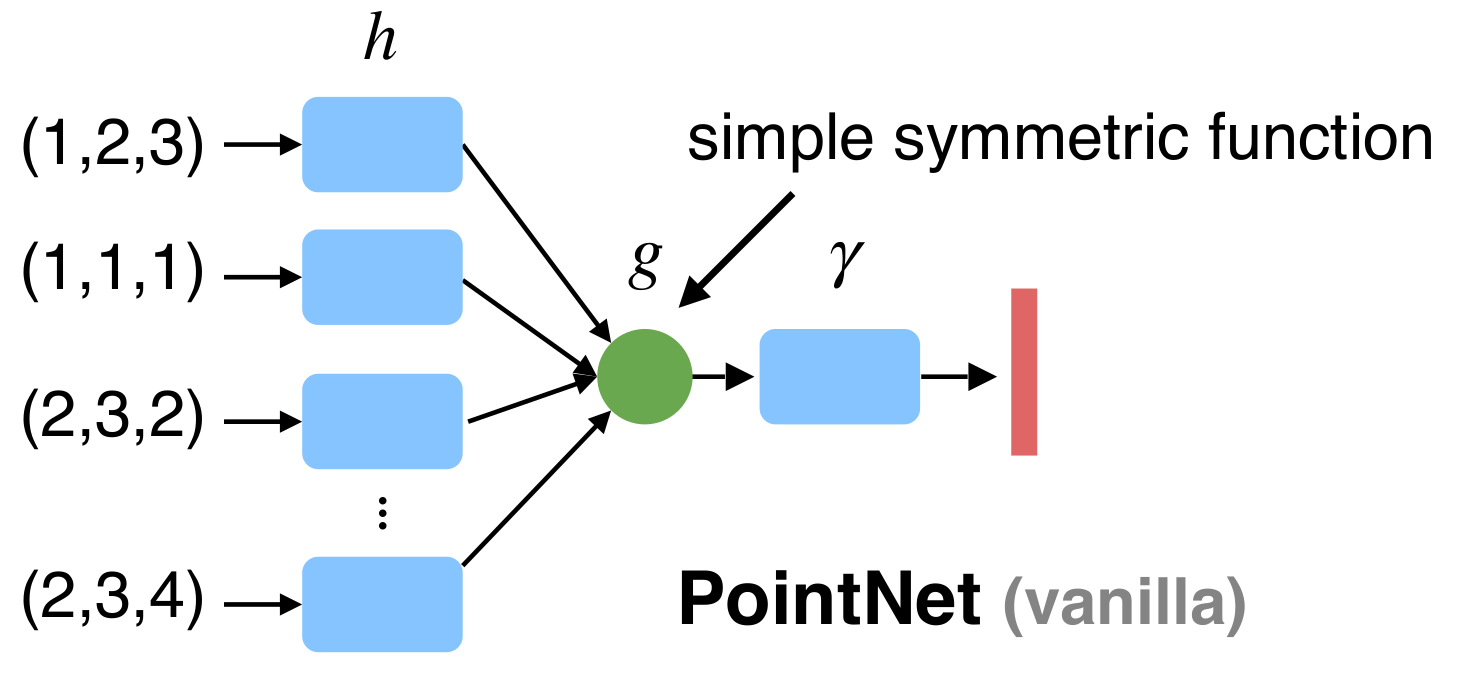
\includegraphics[height=0.45\textheight]{pointnet_vanilla2}
        \caption{Figure from CVPR presentation to \cite{qi2017pointnet}.}
    \end{figure}
    \pnote{
        Erinnerung: Konkatenation von Funktionen kann andere \\
        Funktionen approximieren/darstellen.
        \par
        Konkret können wir mit der konkatenation y o g o h \\
        beliebige symmetrische Funktionen darstellen.
    }
\end{frame}


\begin{frame}[c]{Universal Set Function Approximation}
    \large
    PointNet (vanilla) is a \underline{universal set function approximator}.

    \begin{columns}
        \column{.4\textwidth}
        \begin{greenblock}{Theorem}
            A Hausdorff continuous symmetric function $f: 2^\chi \mapsto \mathbb{R}$ can be arbitrarily approximated by PointNet. \\
        \end{greenblock}
        \column{.4\textwidth}
        \pause
        % $$ \left| f(S) - \underbrace{ \gamma \left( \underset{x_i \in S}{\text{MAX}}\{h(x_i)\} \right)}_{\text{PointNet (vanilla)}} \right| < \varepsilon $$
        $$ \left| f(S) - \underbrace{ \gamma \left( \underset{x_i \in S}{g}\{h(x_i)\} \right)}_{\text{PointNet (vanilla)}} \right| < \varepsilon $$
        with $S \subseteq \mathbb{R}^d$ % and $g :=$ MAX
    \end{columns}
    \vspace{2em}
    For details see \cite{qi2017pointnet} and supplemental material.
    \pnote{
        Bekannt: NN sind allgemeine funktionsapproximatoren \\
        Damit ziemlich trivial: PointNet auch für Permutationen
        \par
        Natürlich braucht eine höhere Genauigkeit mehr Parameter
        \par
        Hausdorff: Topologischer Raum mit disjunkten Nachbarschaften
    }
\end{frame}


\begin{frame}[c]{Basic PointNet Architecture}
    \large
    In practice, both $h$ and $\gamma$ are \textbf{multi-layer perceptrons (MLP)} as generic function approximators.
    Empirically, \textbf{max pooling} provides the best results as symmetric function: \\
    \centering
    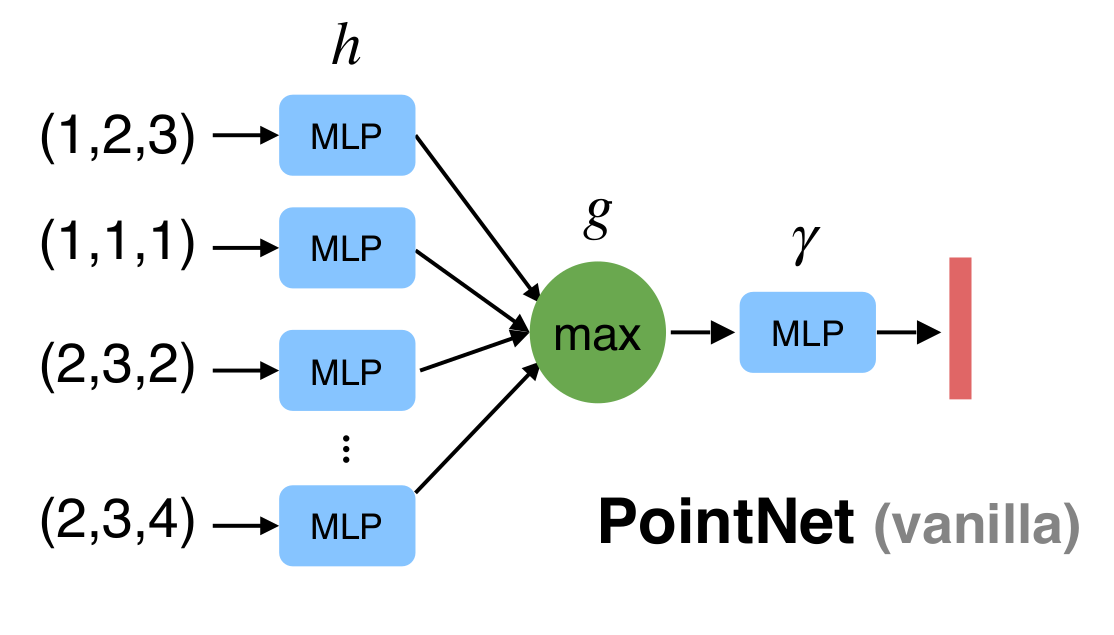
\includegraphics[height=0.6\textheight]{basic_architecture.png}
    \blfootnote{Figure from CVPR presentation to \cite{qi2017pointnet}.}
    \pnote{
        MLP: Dense, Fully-Connected with ReLU \\
        Note that y is shared across all points
        \par
        Andere symmetrische funktionen gehen auch
    }
\end{frame}
% done
\section{Geometric Transformation}
\begin{frame}[c]{Geometric Transformations}
    \large
    \begin{columns}
        \column{0.45\textwidth}
        In particular, point cloud classification should be invariant to:
        \begin{itemize}
            \item Translation
            \item Rotation
            \item Scaling (Dilation)
        \end{itemize}
        \column{0.5\textwidth}
        \centering
        \begin{figure}
            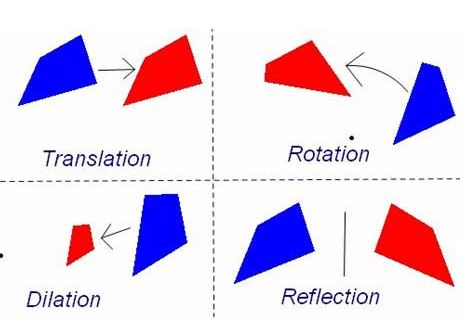
\includegraphics[width=0.8\textwidth]{geometric_transformations}
            \caption{Figure from \cite{BibEntry2019Oct}.}
        \end{figure}
    \end{columns}
    \pnote{
        Relevant: Andere Herausforderung
        \par
        Klassifikation soll unverändert sein über: \\
        - Translation / Bewegung im Raum \\
        - Rotation \\
        - Skalierung \\
        Reflektion sollte bereits über Datensatz enthalten sein
    }
\end{frame}


\begin{frame}[c]{Input Alignment by Transformer Network}
    \begin{columns}
        \column{0.3\textwidth}
        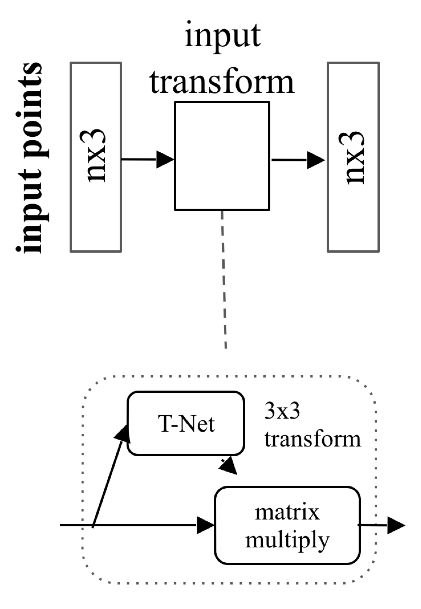
\includegraphics[height=0.7\textheight]{p37_34}
        \column{0.6\textwidth}
        \large
        \pause
        \begin{greenblock}{Solution}
            Have a transformer network (T-Net) figure out data-dependent
            transformations. \\
            \vspace{1em}
            A T-Net is a PointNet (vanilla) with a matrix as output.
        \end{greenblock}
        \vspace{1em}

        \pause
        Additionally, regularize matrix close to orthogonal: $$ L_{reg} = || I - AA^T||_F^2 $$

    \end{columns}
    \blfootnote{Figure from CVPR presentation to \cite{qi2017pointnet}.}
    \pnote{
        Grundidee: Eingabe Normalisieren \\
        Für Point Cloud, Transformation nur Matrixmult
        \par
        PointNet: symmetrisch allgemeiner Funktionsapproximator
        \par
        Verwendung, um datenabhängige Transformationsmatrix \\
        (Normalisierung auf Kanonischen 1-Cube) zu generieren.
    }
\end{frame}


\begin{frame}[c]{Effects of T-Net and Regularization}
    \begin{columns}
        \column{0.6\textwidth}
        \begin{figure}
            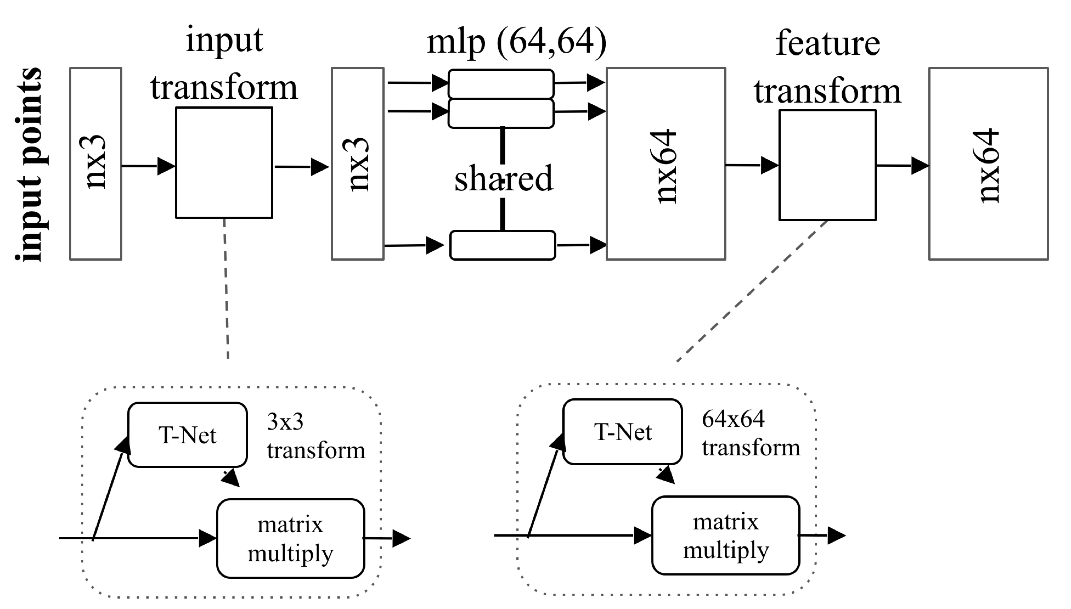
\includegraphics[width=\textwidth,trim=0 10 0 20,clip]{p43_51}
            \caption{Figure from CVPR presentation to \cite{qi2017pointnet}.}
        \end{figure}
        \Large
        \column{0.4\textwidth}
        \pause
        \begin{table}[!ht]
    \centering
    % \resizebox{0.3\textwidth}{!}{%
    \begin{tabular}{l|c}
        Transform & accuracy \\ \hline \hline
        none & 87.1 \\ \hline

        input (3x3) & 87.9 \\
        feature (64x64) & 86.9 \\
        feature (64x64) + reg. & 87.4 \\ \hline

        both & \textbf{89.2}
    \end{tabular}% }
    \caption{
        \textbf{Effects of input feature transforms.} Based on overall classification accuracy on the ModelNet40 \cite{wu20153d} test set.
        Table from \cite{qi2017pointnet}.
    } \label{table:transforms}
\end{table}

    \end{columns}
    \pnote{
        Wir wollen auch mehr als nur die Eingabe Normalisieren \\
        Konkret: Lokaler Feature Vektor  größe 64
    }
\end{frame}

  % done
\section{Structure Visualization}


\begin{frame}[c]{Structure Visualization with dotviz}
    \centering
    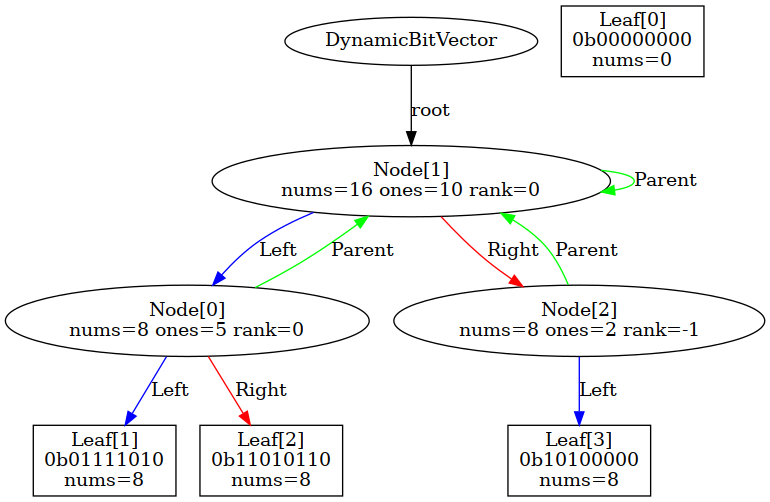
\includegraphics[height=0.75\textheight]{dot_simple}
\end{frame}
%done
\section{Results}
% \begin{frame}[c]{Results on Object Classification}
%     \todo{Picture of input/output}
% \end{frame}
\begin{frame}[c]{Results on Object Classification}
    \begin{columns}
        \centering
        \column{0.7\textwidth}
        \begin{table}[!ht]
    % 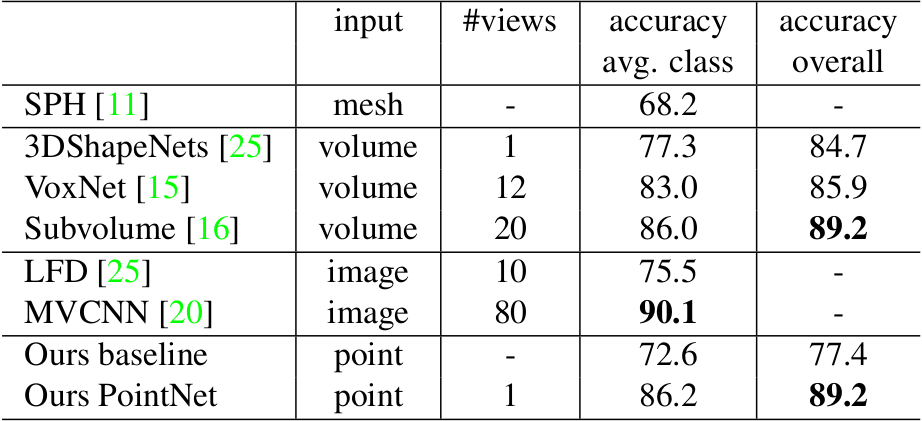
\includegraphics[width=0.5\textwidth]{modelnet}
    \normalsize
    \begin{tabular}{l|c|c|c|c}
        & input & \#views & accuracy & accuracy \\
        & & & avg. class & overall \\ \hline
        SPH \cite{kazhdan2003rotation} & mesh & - & 68.2 & - \\ \hline

        3DShapeNets \cite{wu20153d}     & volume & 1 & 77.3 & 84.7 \\
        VoxNet \cite{maturana2015voxnet} & volume & 12 & 83.0 & 85.9 \\
        Subvolume \cite{qi2016volumetric} & volume & 20 & 86.0 & \textbf{89.2} \\ \hline

        LFD \cite{wu20153d} & image & 10 & 75.5 & - \\
        MVCNN \cite{su2015multi} & image & 80 & \textbf{90.1} & - \\ \hline

        Ours baseline & point & - & 72.6 & 77.4 \\
        Ours PointNet & point & 1 & 86.2 & \textbf{89.2} \\
    \end{tabular}
    \caption{
        \textbf{Classification results on ModelNet40.}
        PointNet achieves state-of-the-art among deep nets on 3D input.
        % Our net achieves
        % state-of-the-art among deep nets on 3D input." Table and caption taken
        % from \cite{qi2017pointnet}. \todo{rewrite in own words}
        Table from \cite{qi2017pointnet}.
    } \label{table:modelnet}
\end{table}

    \end{columns}
    \pnote{In Klassifikation wurde SOTA erreicht.}
\end{frame}


\begin{frame}[c]{Visualization of Object Part Segmentation}
    \begin{columns}
        \column{0.1\textwidth}
        \column{0.7\textwidth}
        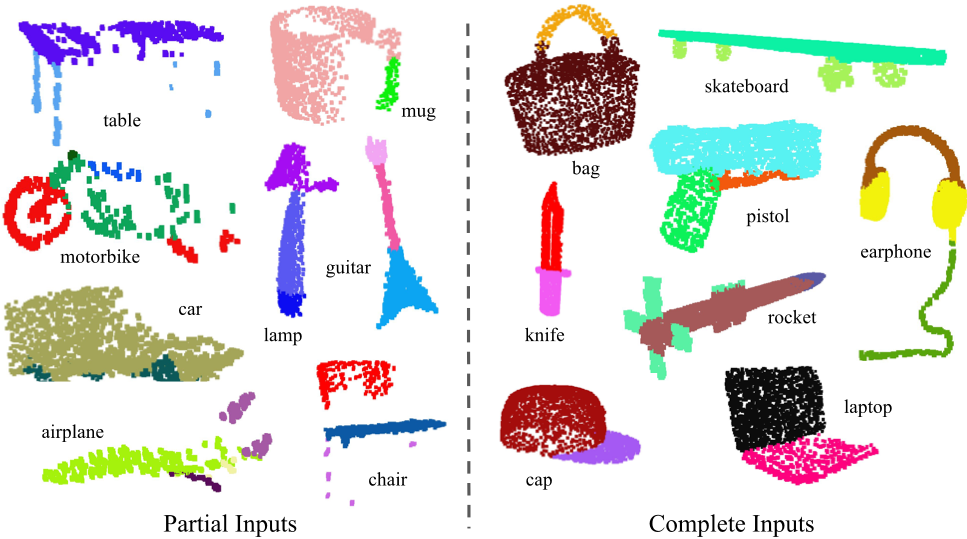
\includegraphics[height=0.75\textheight]{p46_55}
        \column{0.2\textwidth}
        \color{ocre}{Figure from \cite{qi2017pointnet}.}
    \end{columns}
    \pnote{Andere Aufgabe: Segmentieren von (partiellen) Eingaben}
\end{frame}


\begin{frame}[c]{Results on Object Part Segmentation}
    \begin{figure}
        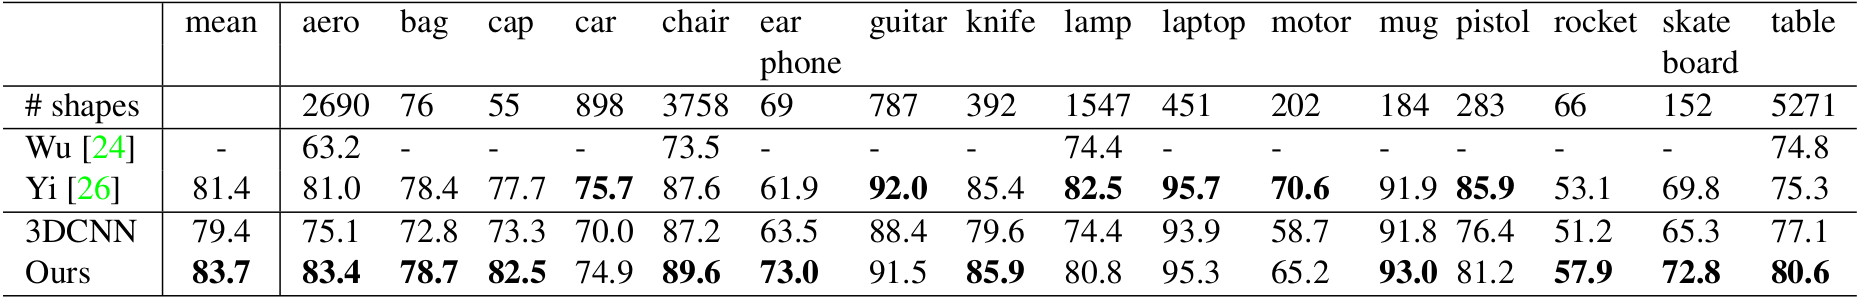
\includegraphics[width=\textwidth]{shapenet}
        \caption{
            \textbf{Segmentation results on ShapeNet part dataset.} The metric
            used is mIoU(\%) on points. Figure/Table from \cite{qi2017pointnet}.}
    \end{figure}
    \pnote{
        Hier wurde eine neue SOTA gesetzt
    }
\end{frame}

\begin{frame}[c]{Semantic Scene Parsing}
    % \begin{figure}[htb]
    \centering % <-- added
    \begin{subfigure}{0.25\textwidth}
        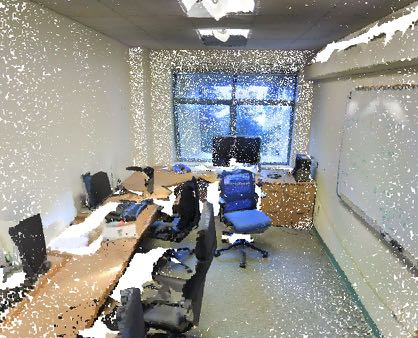
\includegraphics[width=\linewidth]{p48_58}
    \end{subfigure}\hfil % <-- added
    \begin{subfigure}{0.25\textwidth}
        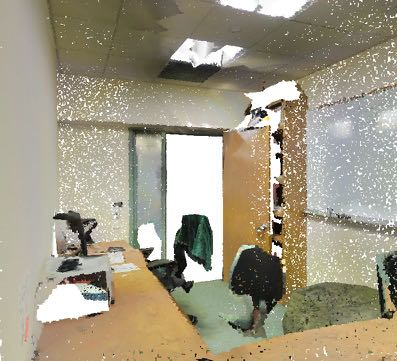
\includegraphics[width=\linewidth]{p48_59}
    \end{subfigure}\hfil % <-- added
    \begin{subfigure}{0.25\textwidth}
        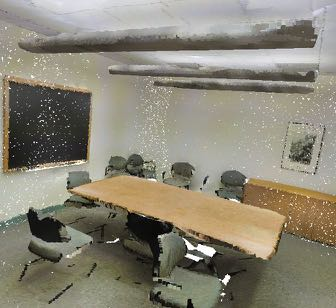
\includegraphics[width=\linewidth]{p48_61}
    \end{subfigure}

    \medskip
    \begin{subfigure}{0.25\textwidth}
        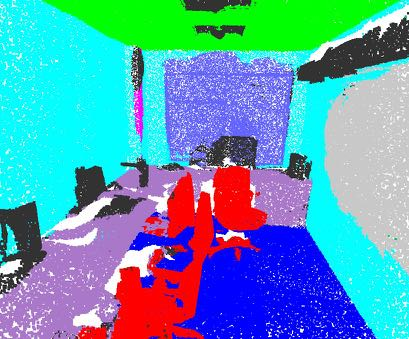
\includegraphics[width=\linewidth]{p48_57}
    \end{subfigure}\hfil % <-- added
    \begin{subfigure}{0.25\textwidth}
        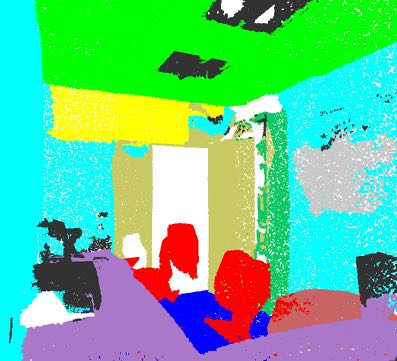
\includegraphics[width=\linewidth]{p48_60}
    \end{subfigure}\hfil % <-- added
    \begin{subfigure}{0.25\textwidth}
        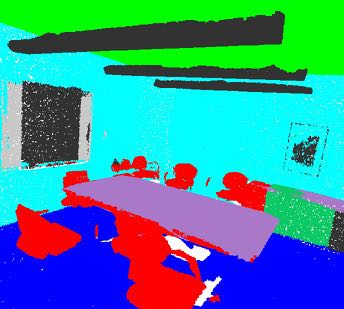
\includegraphics[width=\linewidth]{p48_62}
    \end{subfigure}
    \caption{Figures from \cite{qi2017pointnet}.}
\end{figure}


    \Large
    \begin{columns}
        \column{0.15\textwidth}
        \begin{itemize}
            \item Input
                \vspace{3em}
            \item Output
        \end{itemize}
        \column{0.2\textwidth}
        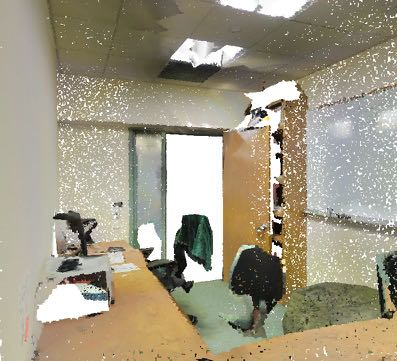
\includegraphics[width=\textwidth]{p48_59} \\
        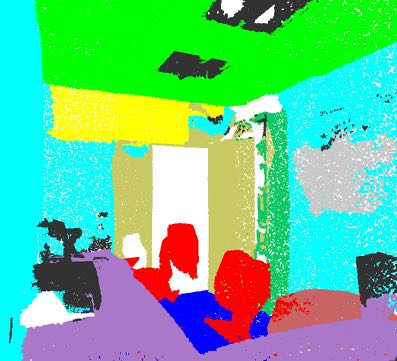
\includegraphics[width=\textwidth]{p48_60}
        \column{0.22\textwidth}
        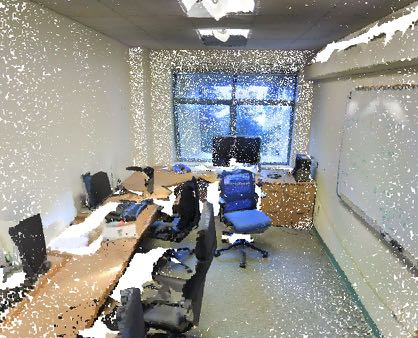
\includegraphics[width=\textwidth]{p48_58} \\
        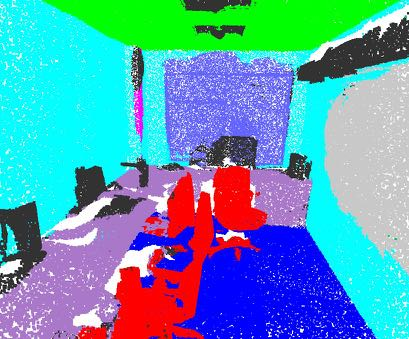
\includegraphics[width=\textwidth]{p48_57}
        \column{0.2\textwidth}
        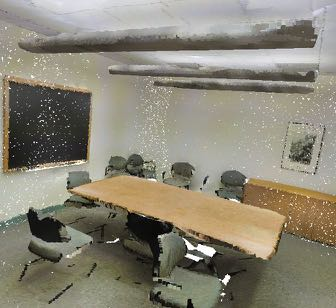
\includegraphics[width=\textwidth]{p48_61} \\
        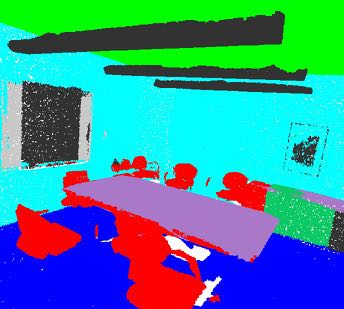
\includegraphics[width=\textwidth]{p48_62}
    \end{columns}
    \blfootnote{Figures from \cite{qi2017pointnet}.}
\end{frame}


\begin{frame}[c]{Robustness to Data Corruption}
    % \begin{figure}[!t]
    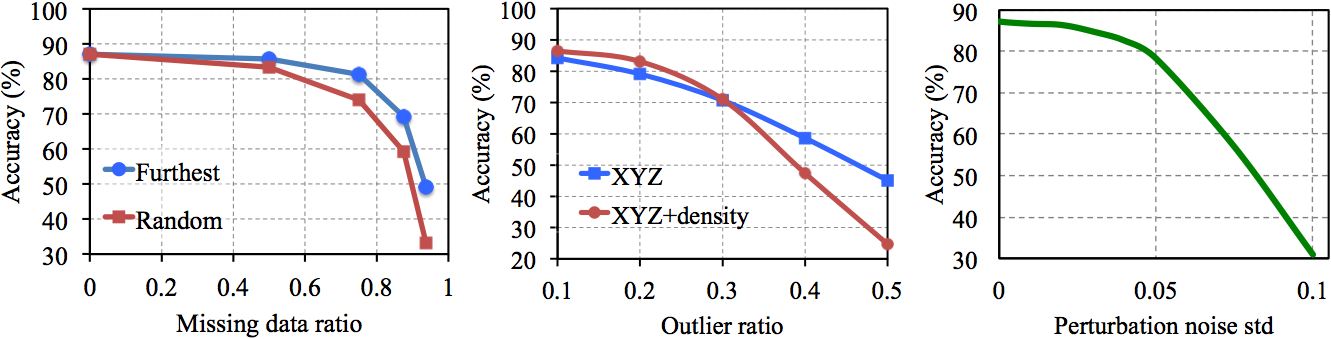
\includegraphics[width=\textwidth]{p51_65}
    \caption{
        \textbf{Robustness tests visualization.}
        Accuracy measured is overall classification accuracy on the ModelNet40
        test set. Left: Point deletion based on different sampling strategies,
        random and furthest sampling, up to the 1024 original points. Middle:
        Insertion of uniformly scattered outliers in the canonicalized unit
        sphere of the original shape. Right: Adding perturbation in the form of
        Gaussian noise with mean 0 to each point in the unit sphere independently.
        Figure from \cite{qi2017pointnet}.
        % The metric is overall classification
        % accuracy on ModelNet40 test set. Left: Delete points. Furthest means
        % the original 1024 points are sampled with furthest sampling. Middle:
        % Insertion. Outliers uniformly scattered in the unit sphere. Right:
        % Perturbation. Add Gaussian noise to each point independently." Figure
        % and caption taken from \cite{qi2017pointnet}. \todo{rewrite in own words}
    } \label{fig:robustness}
\end{figure}



    \begin{figure}
        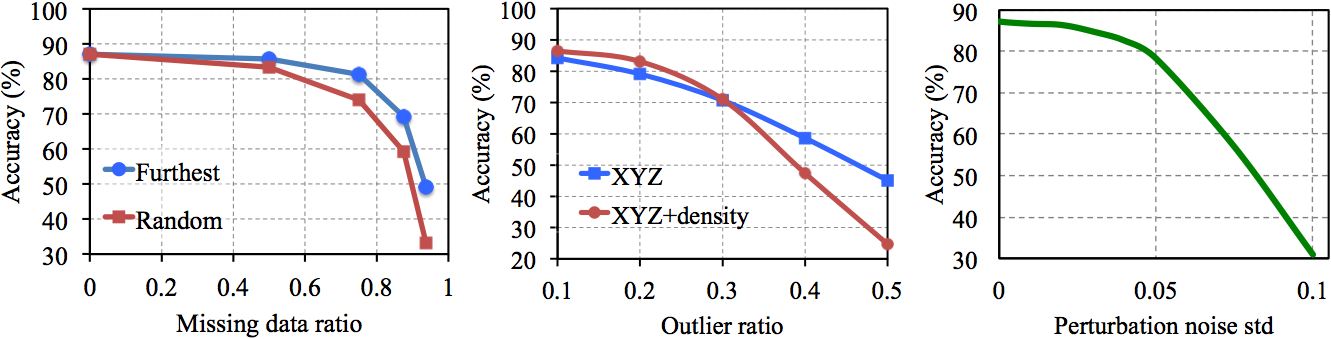
\includegraphics[width=\textwidth]{p51_65}
        \caption{
            \textbf{Robustness tests.}
            Accuracy measured on ModelNet40.
            Figure from \cite{qi2017pointnet}.
        }
    \end{figure}
    \pnote{
        Sehr Robust gegenüber dem: \\
        - Löschen von einzelnen Punkten \\
        - hinzufügen von Ausreißern \\
        - hinzufügen von extremen Rauschen \\
        \par
        Also allgemeinen störungen in Daten. \\
        Next: Anschauen woran das liegt.
    }
\end{frame}


\begin{frame}[c]{Robustness in comparison}
    \Large
    \begin{columns}
        \column{0.5\textwidth}
        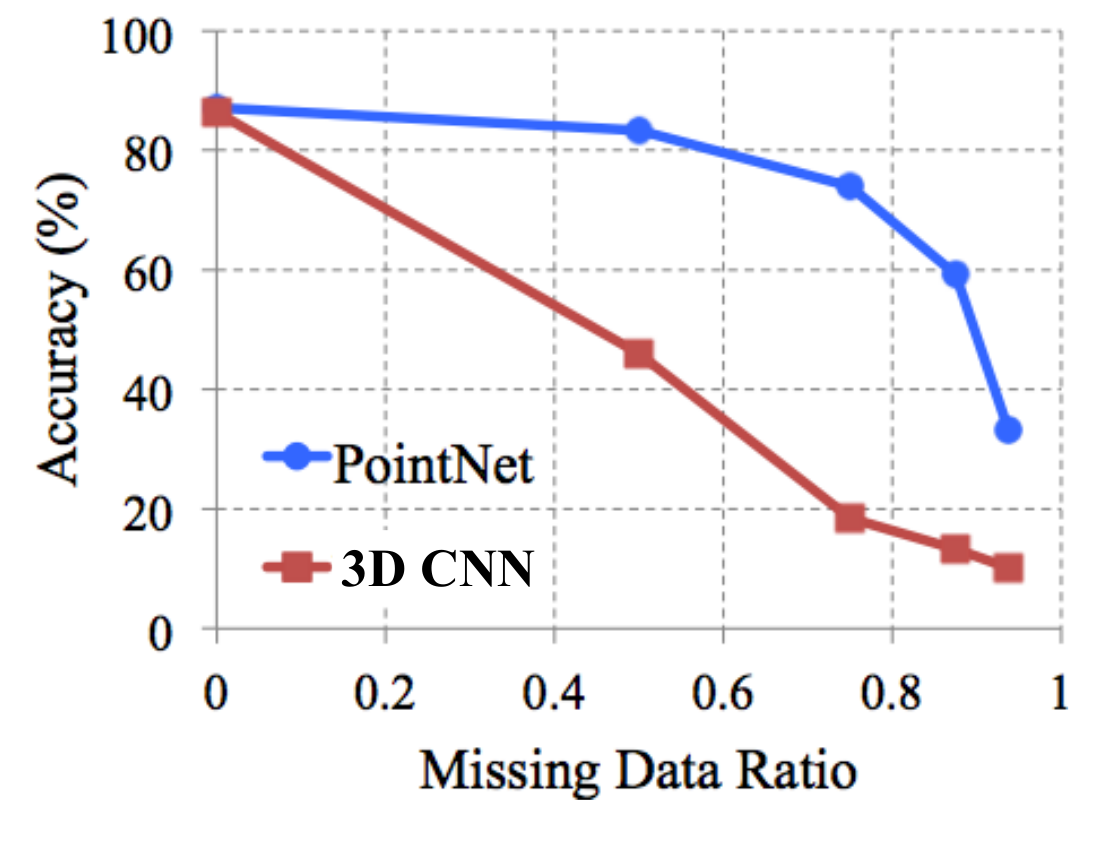
\includegraphics[height=0.7\textheight]{robustness_comp}
        \column{0.3\textwidth}
        Q: Why is PointNet so robust to missing data?
    \end{columns}
    \blfootnote{\textbf{Robustness in comparison with 3D CNN.} Figure from CVPR presentation to \cite{qi2017pointnet}.}
\end{frame}
    % done
\section{Visualization}
\begin{frame}[c]{Visualizing Global Point Cloud Features}
    \Large
    % \begin{itemize}
    %     \item Picture of Architectural overview
    %     \item contributing to global feature: critical points
    %     \item visualizisations, extend to upper bound shape
    % \end{itemize}
    \centering
    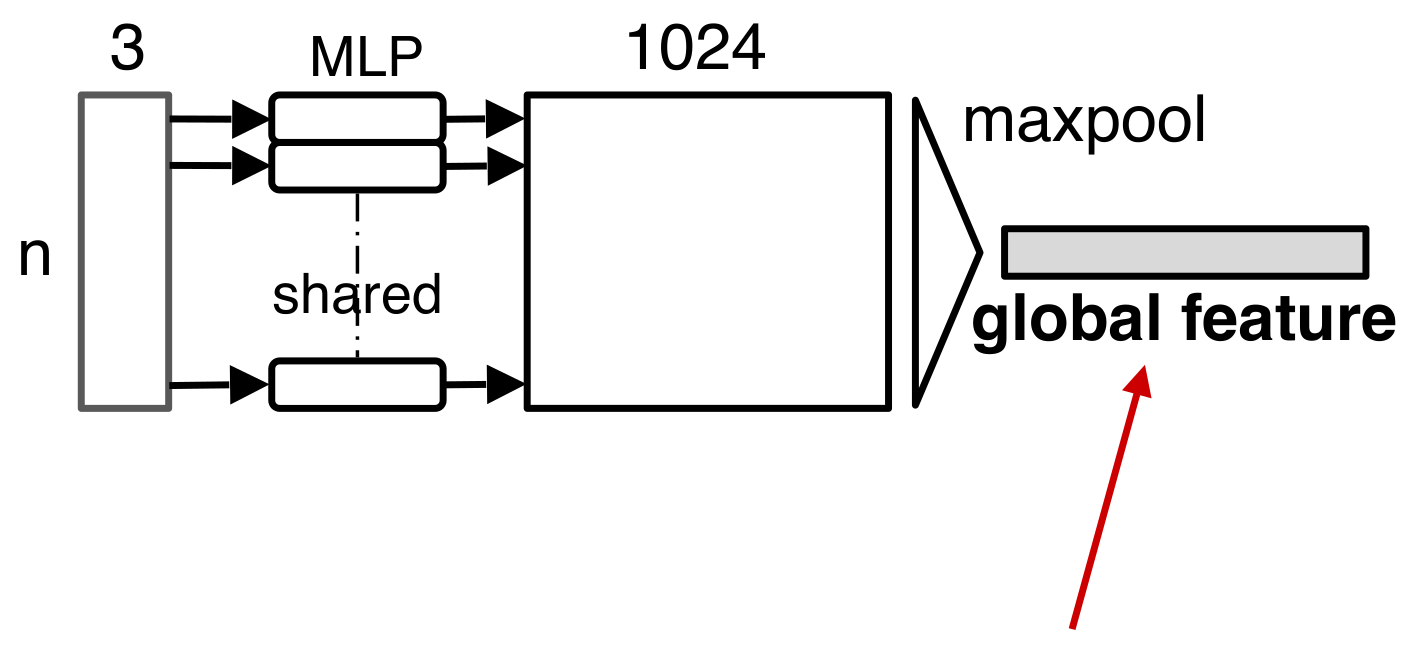
\includegraphics[width=0.55\textwidth]{sympool} \\
    Which points \underline{contribute} to the global feature vector? (\textbf{critical points}) \\
    Which additional points \underline{won't} affect the global feature vector? (\textbf{upper bound}) \\
    \blfootnote{Figure from CVPR presentation to \cite{qi2017pointnet}.}
    \pnote{
        Welche Punkte beeinflussen den Global Feature vektor? \\
        Welche kann man hinzufügen, ohne?
        \par
        Es sollte klar sein, dass nicht alle beitragen werden \\
        aufgrund von max pooling
    }
\end{frame}


\begin{frame}[c]{Visualizing Global Point Cloud Features}
    \centering
    \Large
    \begin{columns}
        \column{0.3\textwidth}
        \begin{itemize}
            \item Original Shape
                \vspace{2.5em}
            \item Critical Point Set
                \vspace{2.5em}
            \item Upper Bound Set
        \end{itemize}
        \column{0.6\textwidth}
        % trim=left bottom right top, clip
        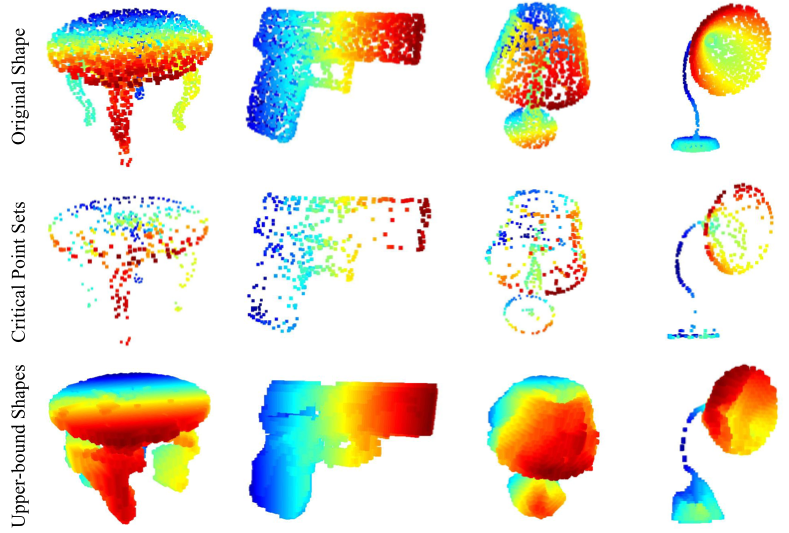
\includegraphics[height=0.7\textheight,trim=40 0 0 0,clip]{p56_68}
    \end{columns}
    \blfootnote{Figure from \cite{qi2017pointnet}.}
    \pnote{
        kritischen Punkte bilden ungefähr ursprüngliche Form \\
        Obere Schranke füllt zwischenräume
        \par
        Erinnerung an Robustheit ggü fehlenden Punkten
    }
\end{frame}


\begin{frame}[c]{Visualizing Global Point Cloud Features (Not in Training)}
    \centering
    \Large
    \begin{columns}
        \column{0.3\textwidth}
        \begin{itemize}
            \item Original Shape
                \vspace{2.5em}
            \item Critical Point Set
                \vspace{2.5em}
            \item Upper Bound Set
        \end{itemize}
        \column{0.6\textwidth}
        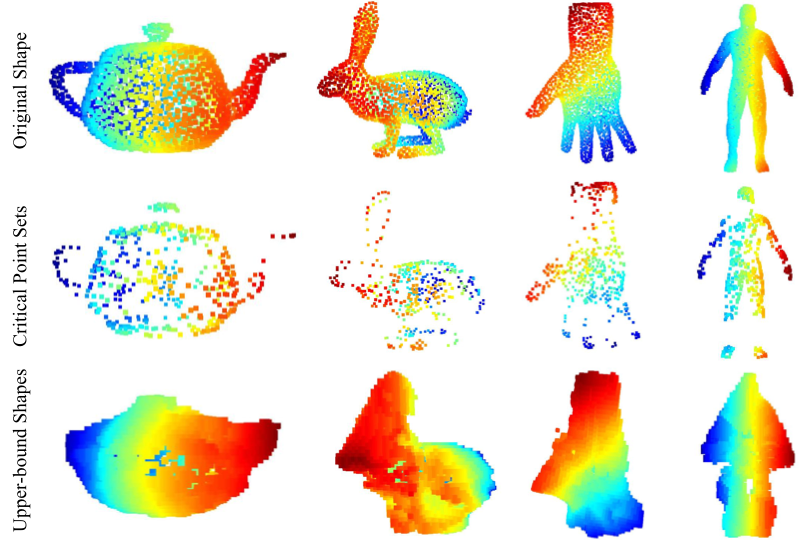
\includegraphics[height=0.7\textheight,trim=40 0 0 0,clip]{p57_69}
    \end{columns}
    \blfootnote{Figure from \cite{qi2017pointnet}.}
    \pnote{
        OOS = Out Of Specification \\
        Also nicht im Trainingsdatensatz enthaltene. \\
        Hier gehen teilweise dinge kaputt
        \par
        Erkenntnis: verallgemeinert gut
    }
\end{frame}


\begin{frame}[c]{Approach to Features Visualization}
    \centering
    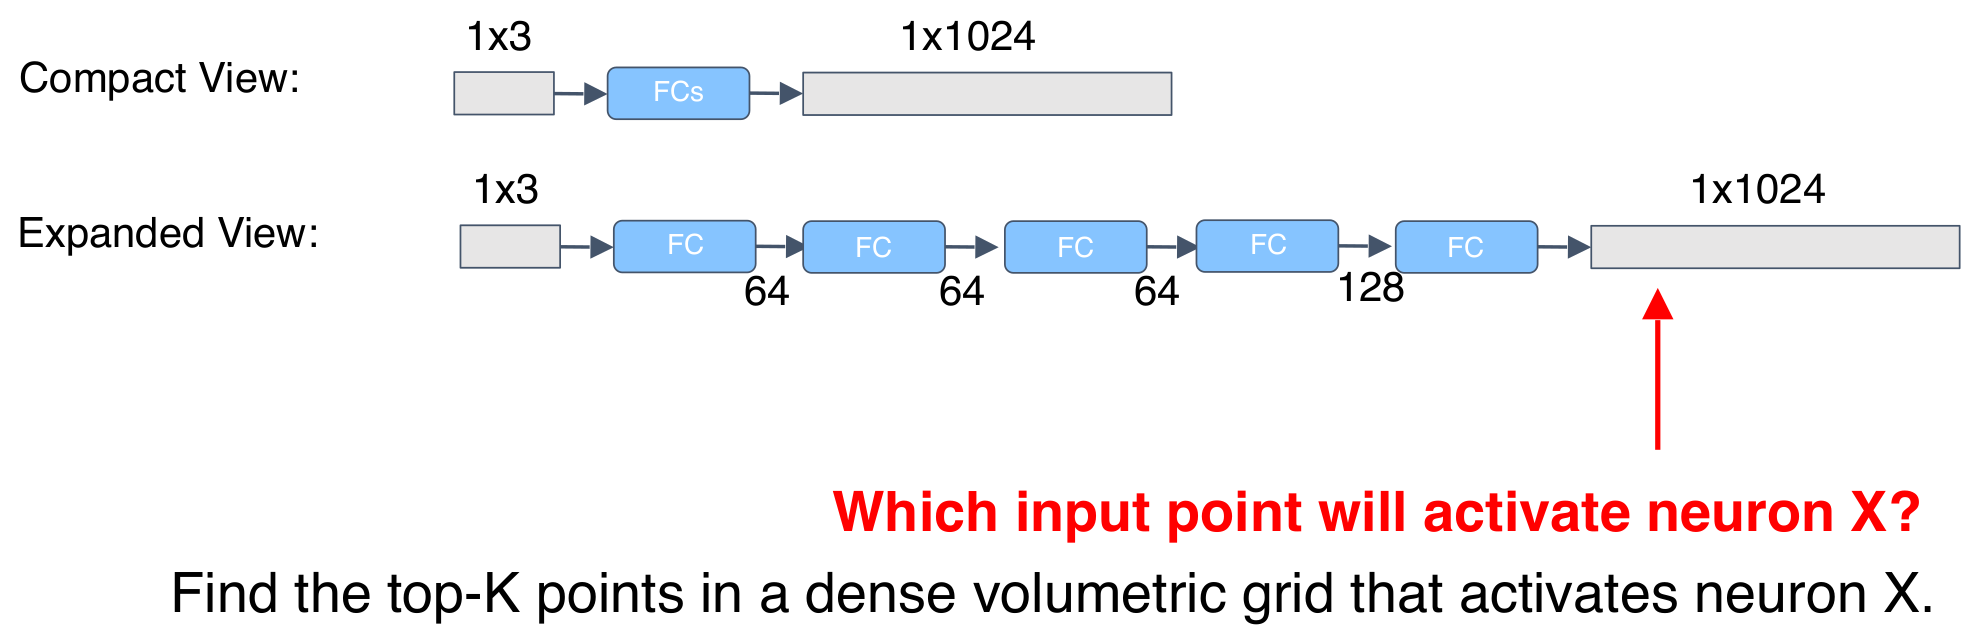
\includegraphics[width=\textwidth]{activation}
    \blfootnote{Figure from CVPR presentation to \cite{qi2017pointnet}.}
    \pnote{
        Visualisieren, was einzelne globale Features aktiviert
    }
\end{frame}


\begin{frame}[c]{Selective Visualization of Activation Features}
    \large
    \centering
    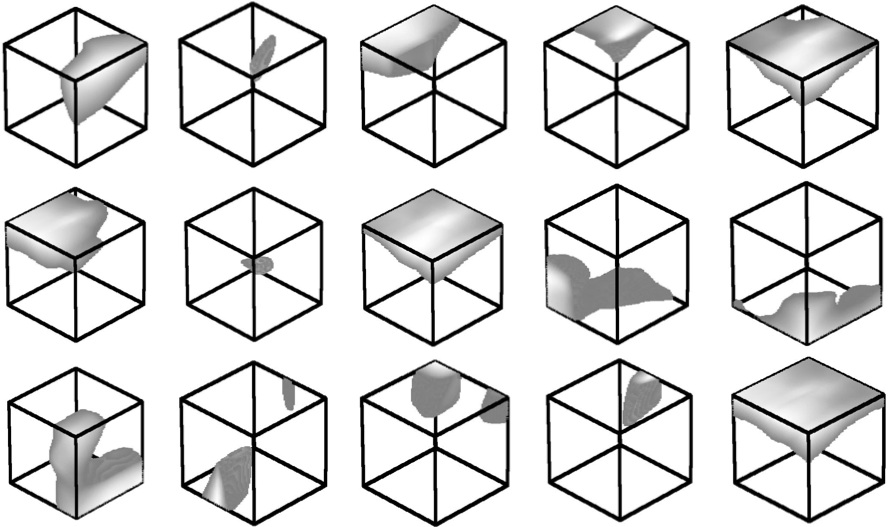
\includegraphics[height=0.7\textheight]{p68_80}
    \blfootnote{Figure from \cite{qi2017pointnet}.}
    \pnote{
        15 zufällig ausgewählte Features (der 1024) \\
        Man sieht, wie erwartet: räumliche Abdeckung
    }
\end{frame}
%done
\section{Impact}
\begin{frame}[c]{Derivative Works of PointNet}
    
\includegraphics[width=\textwidth]{impact}
    \large
    \pause
    Core architecture ideas were adapted in:
    \begin{multicols}{2}
        \begin{itemize}
            \item A sift-like network module \cite{jiang2018sift}
            \item Similarity group proposal network \cite{wang2018sgpn}
            \item Point cloud upsampling \cite{yu2018pu}
            \item Application to Neuroanatomy \cite{gutierrez2018deep}
            \item Frustum pointnets \cite{qi2018frustum}
            \item Pointcnn \cite{li2018pointcnn}
            \item many more ...
        \end{itemize}
    \end{multicols}
    \pnote{
        Auswirkungen von PointNet erstmal nicht wenig \\
        Anfang schreiben: ~7300 \\
        Immernoch höchst relevant
    }
\end{frame}

\begin{frame}[c]{Derivative Works of PointNet II}
    \large
    \begin{multicols}{2}
        PointNet has been used as a module in:
        \begin{itemize}
            \item PointNet++~\cite{qi2017pointnet++}
            \item SyncSpecCNN~\cite{yi2017syncspeccnn}
            \item VoxelNet~\cite{zhou2018voxelnet}
            \item ...
        \end{itemize}
        \begin{figure}
            % 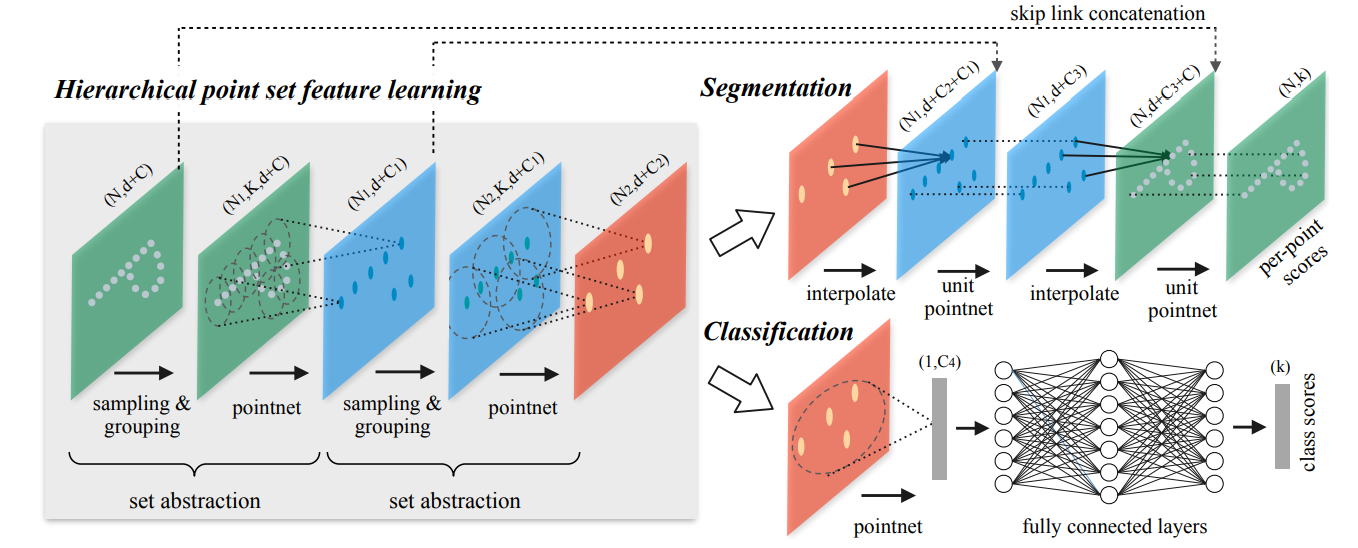
\includegraphics[width=0.5\textwidth]{pointnet_plusplus}
            \includegraphics[width=0.5\textwidth]{pointnet++_architecture}
            \caption{Architecture of PointNet++ with highlighted PointNet layers. Figure adapted from PointNet++~\cite{qi2017pointnet++}}
        \end{figure}
    \end{multicols}
    \pnote{
        Was auch passiert ist, ist dass es als modul / layer  \\
        verwendet wird
    }
\end{frame}

     % done
\section{Conclusion}


\begin{frame}[c]{Review}
    We made substantial Progress!
\end{frame}

\begin{frame}[c]{Next Steps}
    There's a bunch of stuff still left to do:
    \begin{itemize}[<+(1)->]
        \item Deployment of the newly implemented features
        \item Adapt design to current KIT corporate design
        \item Finish dynamic \mintinline{python}{PersonForms} implementation
        \item Login with non-unique identifiers (EPPN)
        \item Advanced User Administration of Accounts
        \item Realizing Projects through Storage API-Access
        \item ...
    \end{itemize}
\end{frame}


 % done

% \section{Results}

\begin{frame}[c]{Results on Object Classification}

\end{frame}

\begin{frame}[c]{Results on Object Part Segmentation}

\end{frame}

\begin{frame}[c]{Results on Semantic Scene Parsing}

\end{frame}

\begin{frame}[c]{Robustness to Data Corruption}

\end{frame}

\begin{frame}[c]{Visualizing Global Point Cloud Features}

\end{frame}

% \section{Introduction}


\begin{frame}[c]{Key Contributions}
The key contributions of the PointNet paper are as follows:
    \begin{itemize}
        \item Design of a novel deep net architecture suitable for unordered point sets in 3D;
        \item Showing how such a net can be trained to perform 3D shape classification, shape part segmentation and scene semantic parsing tasks;
        \item Thorough empirical and theoretical analysis on stability and efficiency of the method;
        % \item Illustration of the 3D features computed by the selected neurons;
        \item Developing intuitive explanations for its performance.
    \end{itemize}
\end{frame}

\subsection{Related Work}
% \subsubsection{Point Cloud Features}
% Ignore
\subsubsection{Deep Learning on 3D Data}

\begin{frame}[c]{Deep Learning on 3D Data}
    Volumetric CNNs \cite{wu20153d, maturana2015voxnet, qi2016volumetric} apply
conventional 3d convolutional neural networks on voxelized shapes. However,
data sparsity and computation cost of 3d convolution constrain the resolution
of volumetric representation.
\end{frame}

        % Work has been done to mitigate the sparsity problem, but its still challenging for them to process very large point clouds.


\begin{frame}[c]{Multiview-CNNs}

Multiview-CNNs \cite{su2015multi, qi2016volumetric} first render 3D point cloud
in multiple 2D images and apply 2D conv nets for image classification. Given
sufficient computational resources, they achieve dominating performance due to
well-engineered image CNNs. However, it is difficult to extend
image-CNNs to other 3D or point-based tasks.

\end{frame}


\begin{frame}[c]{Feature-based DNNs}

    % \item Spectrial CNNs: spectral CNN on meshes, constrained on manifold meshes and unclear how to extend.
Feature-based DNNs \cite{fang20153d, guo20153d} extract traditional shape
features and convert 3d data to a vector before using a fully connected net for
shape classification. They appear to be limited by the representative power of
the features extracted.

\end{frame}

\subsubsection{Deep Learning on Unordered Sets}

\begin{frame}[c]{Deep Learning on Unordered Sets}
A point cloud is an unordered set of vectors from the data structure point of
view. Most works in deep learning however look at regular input structures like
ordered sequences of images, volumes or points. Unordered point clouds are
rarely considered. One recent work \cite{vinyals2015order} attempts to impose
order on unordered input sets via the attention mechanism. This work focuses on
generic sets and NLP applications, which lacks the characteristics of geometry
in the sets.

\end{frame}

% NOT: spatial transformer nets (T-Nets) related to Transformers \cite{vaswani2017attention}

\subsubsection{Based on PointNet}

\begin{frame}[c]{Based on PointNet}

There exist a number of works explaining, applying and building upon PointNet.
The influence of PointNet can furthermore be seen in the ecosystem of different
implementations and tools for visualization \cite{charlesq342022Jun,
aldipiroli2022Jun, yunxiaoshi2022Jun, Pytorch_Pointnet_Pointnet2}. Different
attempts to explain what PointNet learned \cite{zhang2019explaining,
huang2019claim} exist, and many apply PointNet to different domains and
different problems \cite{thiery2022medical, gutierrez2018deep,
triess2021survey, liang2019multi, zhang2018collaborative, mrowca2018flexible}.
\end{frame}

% as well as blog posts on Medium \cite{DataScienceUB2022Apr, Rigoulet2022Apr, Gonzales2021Dec},

\subsubsection{Derivations of PointNet}

\begin{frame}[c]{Derivations of PointNet}

PointNet, in addition to being successful itself, sees successful use as a
module similar to a convolution layer in more sophisticated neural network
architectures.
% "PointNet is becoming a module similar to a convolution layer and is used directly as the base of many netwoks" according to \cite{zhang2019explaining}.
% "Among them, PointNet is becoming a module similar to a convolution layer and is used directly as the base of many netwoks."
This can best be seen in recent architectures such as PointNet++
\cite{qi2017pointnet++}, VoxNet \cite{maturana2015voxnet}, and Syncspeccnn
\cite{yi2017syncspeccnn}. Moreover, an even larger number of architectures is
being heavily inspired by PointNet or adapts core ideas of the PointNet
architecture \cite{jiang2018sift, wang2018sgpn, yu2018pu, gutierrez2018deep,
qi2018frustum, li2018pointcnn}. This includes architectures both for 3D point
cloud data and traditionally ordered input data structures.

\end{frame}



\subsection{Problem Statement}


\section{Deep Learning on Point Sets}

\subsection{Properties of Point Sets in Rn}

\subsection{PointNet Architecture}

\subsection{Theoretical Analysis}

\begin{frame}[c]{DL on Point Sets}

\end{frame}

% \section{Experiments}

\subsection{3D Object Classification}

\subsection{3D Object Part Segmentation}

\subsection{Architecture Design Analysis}

\subsubsection{Alternative Order-Invariant Methods}
\subsubsection{Effectiveness of Input and Feature Transform}
\subsubsection{Robustness}
\subsubsection{Critical Points and Upper Bound shape}

\subsection{Time and Space Complexity Analysis}


\begin{frame}[c]{Experiments}

\end{frame}

% \section{Erster Abschnitt}

\subsection{Erster Unterabschnitt}
\begin{frame}{Blöcke}
    \begin{contentblock}{Contentblock}
        Farbloser Block mit fetter Überschrift.
    \end{contentblock}
    \begin{columns}
        \column{.3\textwidth}
        \begin{greenblock}{Greenblock}
            Standard (\texttt{block})
        \end{greenblock}
        \column{.3\textwidth}
                \begin{blueblock}{Blueblock}
                    = \texttt{exampleblock}
                \end{blueblock}
                \column{.3\textwidth}
                \begin{redblock}{Redblock}
                    = \texttt{alertblock}
                \end{redblock}
        \end{columns}
        \begin{columns}
            \column{.3\textwidth}
            \begin{brownblock}{Brownblock}
            \end{brownblock}
            \column{.3\textwidth}
            \begin{purpleblock}{Purpleblock}
            \end{purpleblock}
            \column{.3\textwidth}
            \begin{cyanblock}{Cyanblock}
            \end{cyanblock}
        \end{columns}
        \begin{columns}
            \column{.3\textwidth}
            \begin{yellowblock}{Yellowblock}
            \end{yellowblock}
            \column{.3\textwidth}
            \begin{lightgreenblock}{Lightgreenblock}
            \end{lightgreenblock}
            \column{.3\textwidth}
            \begin{orangeblock}{Orangeblock}
            \end{orangeblock}
        \end{columns}
        \begin{columns}
            \column{.3\textwidth}
            \begin{grayblock}{Grayblock}
            \end{grayblock}
            \column{.3\textwidth}
            \column{.3\textwidth}
        \end{columns}
\end{frame}

\subsection{Zweiter Unterabschnitt}
\begin{frame}{Auflistungen}
	Text
	\begin{itemize}
		\item Auflistung\\ Umbruch
		\item Auflistung
		\begin{itemize}
			\item Auflistung
			\item Auflistung
		\end{itemize}
	\end{itemize}
\end{frame}

\section{Zweiter Abschnitt}

\begin{frame}
        Bei Frames ohne Titel wird die Kopfzeile nicht angezeigt, und
    der freie Platz kann für Inhalte genutzt werden.
\end{frame}

\begin{frame}[plain]
    Bei Frames mit Option \texttt{[plain]} werden weder Kopf- noch Fußzeile angezeigt.
\end{frame}

\begin{frame}[t]{Beispielinhalt}
    Bei Frames mit Option \texttt{[t]} werden die Inhalte nicht vertikal zentriert, sondern an der Oberkante begonnen.
\end{frame}


\begin{frame}{Beispielinhalt: Literatur}
    Literaturzitat: \cite{klare2021jss}
\end{frame}


\section{Farben}
%% ----------------------------------------
%% | Test-Folie mit definierten Farben |
%% ----------------------------------------
\begin{frame}{Farbpalette}
\tiny

% GREEN
	\colorbox{kit-green100}{kit-green100}
	\colorbox{kit-green90}{kit-green90}
	\colorbox{kit-green80}{kit-green80}
	\colorbox{kit-green70}{kit-green70}
	\colorbox{kit-green60}{kit-green60}
	\colorbox{kit-green50}{kit-green50}
	\colorbox{kit-green40}{kit-green40}
	\colorbox{kit-green30}{kit-green30}
	\colorbox{kit-green25}{kit-green25}
	\colorbox{kit-green20}{kit-green20}
	\colorbox{kit-green15}{kit-green15}
	\colorbox{kit-green10}{kit-green10}
	\colorbox{kit-green5}{kit-green5}

% BLUE
	\colorbox{kit-blue100}{kit-blue100}
	\colorbox{kit-blue90}{kit-blue90}
	\colorbox{kit-blue80}{kit-blue80}
	\colorbox{kit-blue70}{kit-blue70}
	\colorbox{kit-blue60}{kit-blue60}
	\colorbox{kit-blue50}{kit-blue50}
	\colorbox{kit-blue40}{kit-blue40}
	\colorbox{kit-blue30}{kit-blue30}
	\colorbox{kit-blue25}{kit-blue25}
	\colorbox{kit-blue20}{kit-blue20}
	\colorbox{kit-blue15}{kit-blue15}
	\colorbox{kit-blue10}{kit-blue10}
	\colorbox{kit-blue5}{kit-blue5}

% RED
	\colorbox{kit-red100}{kit-red100}
	\colorbox{kit-red90}{kit-red90}
	\colorbox{kit-red80}{kit-red80}
	\colorbox{kit-red70}{kit-red70}
	\colorbox{kit-red60}{kit-red60}
	\colorbox{kit-red50}{kit-red50}
	\colorbox{kit-red40}{kit-red40}
	\colorbox{kit-red30}{kit-red30}
	\colorbox{kit-red25}{kit-red25}
	\colorbox{kit-red20}{kit-red20}
	\colorbox{kit-red15}{kit-red15}
	\colorbox{kit-red10}{kit-red10}
	\colorbox{kit-red5}{kit-red5}

% GREY
	\colorbox{kit-gray100}{\color{white}kit-gray100}
	\colorbox{kit-gray90}{\color{white}kit-gray90}
	\colorbox{kit-gray80}{\color{white}kit-gray80}
	\colorbox{kit-gray70}{\color{white}kit-gray70}
	\colorbox{kit-gray60}{\color{white}kit-gray60}
	\colorbox{kit-gray50}{\color{white}kit-gray50}
	\colorbox{kit-gray40}{kit-gray40}
	\colorbox{kit-gray30}{kit-gray30}
	\colorbox{kit-gray25}{kit-gray25}
	\colorbox{kit-gray20}{kit-gray20}
	\colorbox{kit-gray15}{kit-gray15}
	\colorbox{kit-gray10}{kit-gray10}
	\colorbox{kit-gray5}{kit-gray5}

% Orange
	\colorbox{kit-orange100}{kit-orange100}
	\colorbox{kit-orange90}{kit-orange90}
	\colorbox{kit-orange80}{kit-orange80}
	\colorbox{kit-orange70}{kit-orange70}
	\colorbox{kit-orange60}{kit-orange60}
	\colorbox{kit-orange50}{kit-orange50}
	\colorbox{kit-orange40}{kit-orange40}
	\colorbox{kit-orange30}{kit-orange30}
	\colorbox{kit-orange25}{kit-orange25}
	\colorbox{kit-orange20}{kit-orange20}
	\colorbox{kit-orange15}{kit-orange15}
	\colorbox{kit-orange10}{kit-orange10}
	\colorbox{kit-orange5}{kit-orange5}

% lightgreen
	\colorbox{kit-lightgreen100}{kit-lightgreen100}
	\colorbox{kit-lightgreen90}{kit-lightgreen90}
	\colorbox{kit-lightgreen80}{kit-lightgreen80}
	\colorbox{kit-lightgreen70}{kit-lightgreen70}
	\colorbox{kit-lightgreen60}{kit-lightgreen60}
	\colorbox{kit-lightgreen50}{kit-lightgreen50}
	\colorbox{kit-lightgreen40}{kit-lightgreen40}
	\colorbox{kit-lightgreen30}{kit-lightgreen30}
	\colorbox{kit-lightgreen25}{kit-lightgreen25}
	\colorbox{kit-lightgreen20}{kit-lightgreen20}
	\colorbox{kit-lightgreen15}{kit-lightgreen15}
	\colorbox{kit-lightgreen10}{kit-lightgreen10}
	\colorbox{kit-lightgreen5}{kit-lightgreen5}

% Brown
	\colorbox{kit-brown100}{kit-brown100}
	\colorbox{kit-brown90}{kit-brown90}
	\colorbox{kit-brown80}{kit-brown80}
	\colorbox{kit-brown70}{kit-brown70}
	\colorbox{kit-brown60}{kit-brown60}
	\colorbox{kit-brown50}{kit-brown50}
	\colorbox{kit-brown40}{kit-brown40}
	\colorbox{kit-brown30}{kit-brown30}
	\colorbox{kit-brown25}{kit-brown25}
	\colorbox{kit-brown20}{kit-brown20}
	\colorbox{kit-brown15}{kit-brown15}
	\colorbox{kit-brown10}{kit-brown10}
	\colorbox{kit-brown5}{kit-brown5}

% Purple
	\colorbox{kit-purple100}{kit-purple100}
	\colorbox{kit-purple90}{kit-purple90}
	\colorbox{kit-purple80}{kit-purple80}
	\colorbox{kit-purple70}{kit-purple70}
	\colorbox{kit-purple60}{kit-purple60}
	\colorbox{kit-purple50}{kit-purple50}
	\colorbox{kit-purple40}{kit-purple40}
	\colorbox{kit-purple30}{kit-purple30}
	\colorbox{kit-purple25}{kit-purple25}
	\colorbox{kit-purple20}{kit-purple20}
	\colorbox{kit-purple15}{kit-purple15}
	\colorbox{kit-purple10}{kit-purple10}
	\colorbox{kit-purple5}{kit-purple5}

% Cyan
	\colorbox{kit-cyan100}{kit-cyan100}
	\colorbox{kit-cyan90}{kit-cyan90}
	\colorbox{kit-cyan80}{kit-cyan80}
	\colorbox{kit-cyan70}{kit-cyan70}
	\colorbox{kit-cyan60}{kit-cyan60}
	\colorbox{kit-cyan50}{kit-cyan50}
	\colorbox{kit-cyan40}{kit-cyan40}
	\colorbox{kit-cyan30}{kit-cyan30}
	\colorbox{kit-cyan25}{kit-cyan25}
	\colorbox{kit-cyan20}{kit-cyan20}
	\colorbox{kit-cyan15}{kit-cyan15}
	\colorbox{kit-cyan10}{kit-cyan10}
	\colorbox{kit-cyan5}{kit-cyan5}

\end{frame}
%% ----------------------------------------
%% | /Test-Folie mit definierten Farben |
%% ----------------------------------------



% \maketitle
% \input{chapters/abstract.tex}
% \section{Introduction}


\begin{frame}[c]{Key Contributions}
The key contributions of the PointNet paper are as follows:
    \begin{itemize}
        \item Design of a novel deep net architecture suitable for unordered point sets in 3D;
        \item Showing how such a net can be trained to perform 3D shape classification, shape part segmentation and scene semantic parsing tasks;
        \item Thorough empirical and theoretical analysis on stability and efficiency of the method;
        % \item Illustration of the 3D features computed by the selected neurons;
        \item Developing intuitive explanations for its performance.
    \end{itemize}
\end{frame}

\subsection{Related Work}
% \subsubsection{Point Cloud Features}
% Ignore
\subsubsection{Deep Learning on 3D Data}

\begin{frame}[c]{Deep Learning on 3D Data}
    Volumetric CNNs \cite{wu20153d, maturana2015voxnet, qi2016volumetric} apply
conventional 3d convolutional neural networks on voxelized shapes. However,
data sparsity and computation cost of 3d convolution constrain the resolution
of volumetric representation.
\end{frame}

        % Work has been done to mitigate the sparsity problem, but its still challenging for them to process very large point clouds.


\begin{frame}[c]{Multiview-CNNs}

Multiview-CNNs \cite{su2015multi, qi2016volumetric} first render 3D point cloud
in multiple 2D images and apply 2D conv nets for image classification. Given
sufficient computational resources, they achieve dominating performance due to
well-engineered image CNNs. However, it is difficult to extend
image-CNNs to other 3D or point-based tasks.

\end{frame}


\begin{frame}[c]{Feature-based DNNs}

    % \item Spectrial CNNs: spectral CNN on meshes, constrained on manifold meshes and unclear how to extend.
Feature-based DNNs \cite{fang20153d, guo20153d} extract traditional shape
features and convert 3d data to a vector before using a fully connected net for
shape classification. They appear to be limited by the representative power of
the features extracted.

\end{frame}

\subsubsection{Deep Learning on Unordered Sets}

\begin{frame}[c]{Deep Learning on Unordered Sets}
A point cloud is an unordered set of vectors from the data structure point of
view. Most works in deep learning however look at regular input structures like
ordered sequences of images, volumes or points. Unordered point clouds are
rarely considered. One recent work \cite{vinyals2015order} attempts to impose
order on unordered input sets via the attention mechanism. This work focuses on
generic sets and NLP applications, which lacks the characteristics of geometry
in the sets.

\end{frame}

% NOT: spatial transformer nets (T-Nets) related to Transformers \cite{vaswani2017attention}

\subsubsection{Based on PointNet}

\begin{frame}[c]{Based on PointNet}

There exist a number of works explaining, applying and building upon PointNet.
The influence of PointNet can furthermore be seen in the ecosystem of different
implementations and tools for visualization \cite{charlesq342022Jun,
aldipiroli2022Jun, yunxiaoshi2022Jun, Pytorch_Pointnet_Pointnet2}. Different
attempts to explain what PointNet learned \cite{zhang2019explaining,
huang2019claim} exist, and many apply PointNet to different domains and
different problems \cite{thiery2022medical, gutierrez2018deep,
triess2021survey, liang2019multi, zhang2018collaborative, mrowca2018flexible}.
\end{frame}

% as well as blog posts on Medium \cite{DataScienceUB2022Apr, Rigoulet2022Apr, Gonzales2021Dec},

\subsubsection{Derivations of PointNet}

\begin{frame}[c]{Derivations of PointNet}

PointNet, in addition to being successful itself, sees successful use as a
module similar to a convolution layer in more sophisticated neural network
architectures.
% "PointNet is becoming a module similar to a convolution layer and is used directly as the base of many netwoks" according to \cite{zhang2019explaining}.
% "Among them, PointNet is becoming a module similar to a convolution layer and is used directly as the base of many netwoks."
This can best be seen in recent architectures such as PointNet++
\cite{qi2017pointnet++}, VoxNet \cite{maturana2015voxnet}, and Syncspeccnn
\cite{yi2017syncspeccnn}. Moreover, an even larger number of architectures is
being heavily inspired by PointNet or adapts core ideas of the PointNet
architecture \cite{jiang2018sift, wang2018sgpn, yu2018pu, gutierrez2018deep,
qi2018frustum, li2018pointcnn}. This includes architectures both for 3D point
cloud data and traditionally ordered input data structures.

\end{frame}



\subsection{Problem Statement}


\section{Deep Learning on Point Sets}

\subsection{Properties of Point Sets in Rn}

\subsection{PointNet Architecture}

\subsection{Theoretical Analysis}

\begin{frame}[c]{DL on Point Sets}

\end{frame}

% % \section{Motivation}
% \begin{frame}[c]{The Need for 3D Deep Learning}
%     \large
%     \begin{figure}
    \captionsetup[subfigure]{labelformat=empty}
    \begin{subfigure}{0.3\textwidth}
        % lidar car visualization
        Robot Perception \\
        \includegraphics[height=0.35\textheight]{p02_6}
        \caption{source: Scott J Grunewald}
    \end{subfigure}
    \hspace{5mm}
    \begin{subfigure}{0.3\textwidth}
        % phone AR
        Augmented Reality \\
        \includegraphics[height=0.35\textheight]{p02_8}
        \caption{source: Google Tango}
    \end{subfigure}
    \hspace{2mm}
    \begin{subfigure}{0.3\textwidth}
        % solidworks 3D objects
        Shape Design \\
        \includegraphics[height=0.35\textheight]{p02_7}
        \caption{source: solidworks}
    \end{subfigure}
    \blfootnote{Figures and captions from CVPR presentation to \cite{qi2017pointnet}.}
\end{figure}

%     \Large
%     \vspace{1em}
%     A number of emerging 3D applications shape the need for 3D deep learning.
%     \pnote{
%         Es entstehen viele Anwendungen die Wahrnehmung  \\
%         oder Interaktion in 3D benötigen.
%         \par
%         - viele Anwendungen im 3D bereich entstehen \\
%         - brauchen Wahrnehmung oder Interaktion in 3D \\
%         - um diese zu bedienen: hoher bedarf \\
%         - spezifisch auf 3D zugeschnitten \\
%         - Erster: PointNet \\
%     }
% \end{frame}


\section{Representation}
\begin{frame}[c]{Common Representations of 3D Data}
    \begin{figure}
    % \captionsetup[subfigure]{labelformat=empty, size=\large, labelfont={black, bf}}
    \captionsetup[subfigure]{labelformat=empty, font={large, color=black}}
    \begin{subfigure}{0.23\textwidth}
        \includegraphics[height=0.35\textheight]{p04_12}
        \caption{Point Cloud}
    \end{subfigure}
    \begin{subfigure}{0.23\textwidth}
        \includegraphics[height=0.35\textheight]{p04_13}
        \caption{Mesh}
    \end{subfigure}
    \begin{subfigure}{0.23\textwidth}
        \includegraphics[height=0.35\textheight]{p04_14}
        \caption{Volumetric}
    \end{subfigure}
    \hspace{1mm}
    \begin{subfigure}{0.23\textwidth}
        \includegraphics[height=0.35\textheight]{p04_15}
        \caption{View Rendering}
    \end{subfigure}
    \blfootnote{Figures and captions (partially) from CVPR presentation to \cite{qi2017pointnet}.}
\end{figure}

    \Large
    \vspace{1em}
    Contrary to 2D, 3D has many different popular representations.
    \pnote{Auszug an Beispielen}
\end{frame}


\begin{frame}[c]{Canonical Representation: Point Cloud}
    \large
    \begin{columns}
        \column{0.32\textwidth}
        \begin{itemize}
            \item Point cloud is close to \textbf{raw depth sensor data}
            \item Point cloud is \textbf{canonical} (easy conversion from and to other representations)
        \end{itemize}
        \color{ocre}
        \normalsize
        \vspace{2em}
        Individual figures from CVPR presentation to \cite{qi2017pointnet}
        \column{0.68\textwidth}
        \includegraphics[height=0.75\textheight]{canonical}
    \end{columns}
    \pnote{
        - Am nächsten zu ursprünglichen Tiefendaten\\
        - Kanonische Form: andere lassen sich einfach umwandeln \\
        Allerdings: wenig Arbeit zu Point Cloud Features
    }
\end{frame}


% \begin{table}[!ht]
    \small
    \begin{tabular}{l|c|cccccccccccccccc}
        & mean & aero & bag & cap & car & chair & ear & guitar & knife & lamp & laptop & motor & mug & pistol & rocket & skate & table \\
        & & & & & & & phone & & & & & & & & & board & \\ \hline
        \# shapes & & 2690 & 76 & 55 & 898 & 3758 & 69 & 787 & 392 & 1547 & 451 & 202 & 184 & 283 & 66 & 152 & 5271 \\ \hline
        Wu \cite{wu2014interactive} & - & 63.2 & - & - & - & 73.5 & - & - & - & 74.4 & - & - & - & - & - & - & 74.8 \\
        Yi \cite{yi2016scalable} & 81.4 & 81.0 & 78.4 & 77.7 & \textbf{75.7} & 87.6 & 61.9 & \textbf{92.0} & 85.4 & \textbf{82.5} & \textbf{95.7} & \textbf{70.6} & 91.9 & \textbf{85.9} & 53.1 & 69.8 & 75.3 \\ \hline
        3DCNN & 79.4 & 75.1 & 72.8 & 73.3 & 70.0 & 87.2 & 63.5 & 88.4 & 79.6 & 74.4 & 93.9 & 58.7 & 91.8 & 76.4 & 51.2 & 65.3 & 77.1 \\
        Ours & \textbf{83.7} & \textbf{83.4} & \textbf{87.7} & \textbf{82.5} & 74.9 & \textbf{89.6} & \textbf{73.0} & 91.5 & \textbf{85.9} & 80.8 & 95.3 & 65.2 & \textbf{93.0} & 81.2 & \textbf{57.9} & \textbf{72.8} & \textbf{80.6}
    \end{tabular}
    \caption{
        \textbf{Segmentation results on ShapeNet part dataset.} The metric used is mIoU(\%) on points.
        As a baseline, we compare with a 3D fully convolutional
        network pipeline proposed by us as well as two
        traditional methods \cite{wu2014interactive} and
        \cite{yi2016scalable}.
        We observe that PointNet achieved a new state-of-the-art
        in mIoU. Table from \cite{qi2017pointnet}.
    } \label{table:shapenet}
\end{table}

% \input{chapters/properties.tex}
% \section{Structure Visualization}


\begin{frame}[c]{Structure Visualization with dotviz}
    \centering
    \includegraphics[height=0.75\textheight]{dot_simple}
\end{frame}

% \input{chapters/analysis.tex}
% \begin{table}[!ht]
    % \includegraphics[width=0.5\textwidth]{modelnet}
    \normalsize
    \begin{tabular}{l|c|c|c|c}
        & input & \#views & accuracy & accuracy \\
        & & & avg. class & overall \\ \hline
        SPH \cite{kazhdan2003rotation} & mesh & - & 68.2 & - \\ \hline

        3DShapeNets \cite{wu20153d}     & volume & 1 & 77.3 & 84.7 \\
        VoxNet \cite{maturana2015voxnet} & volume & 12 & 83.0 & 85.9 \\
        Subvolume \cite{qi2016volumetric} & volume & 20 & 86.0 & \textbf{89.2} \\ \hline

        LFD \cite{wu20153d} & image & 10 & 75.5 & - \\
        MVCNN \cite{su2015multi} & image & 80 & \textbf{90.1} & - \\ \hline

        Ours baseline & point & - & 72.6 & 77.4 \\
        Ours PointNet & point & 1 & 86.2 & \textbf{89.2} \\
    \end{tabular}
    \caption{
        \textbf{Classification results on ModelNet40.}
        PointNet achieves state-of-the-art among deep nets on 3D input.
        % Our net achieves
        % state-of-the-art among deep nets on 3D input." Table and caption taken
        % from \cite{qi2017pointnet}. \todo{rewrite in own words}
        Table from \cite{qi2017pointnet}.
    } \label{table:modelnet}
\end{table}

% \input{chapters/comparison.tex}
% \section{Conclusion}


\begin{frame}[c]{Review}
    We made substantial Progress!
\end{frame}

\begin{frame}[c]{Next Steps}
    There's a bunch of stuff still left to do:
    \begin{itemize}[<+(1)->]
        \item Deployment of the newly implemented features
        \item Adapt design to current KIT corporate design
        \item Finish dynamic \mintinline{python}{PersonForms} implementation
        \item Login with non-unique identifiers (EPPN)
        \item Advanced User Administration of Accounts
        \item Realizing Projects through Storage API-Access
        \item ...
    \end{itemize}
\end{frame}






\appendix
\beginbackup
% \begin{frame}[c,fragile,allowframebreaks]{Sources}
% % \bibliographystyle{plainnat}
% \bibliographystyle{plain}
% % \bibliographystyle{ieeetr}
% \bibliography{references}
% \end{frame}


    % \bibliography{references.bib}

% \begin{frame}[c,fragile,allowframebreaks]{Sources}
%     \bibliographystyle{plain}
%     \bibliography{references.bib}
% \end{frame}


\begin{frame}[c,fragile,allowframebreaks]{Sources}
    \printbibliography
\end{frame}

\section{Multi-Layer Perceptron}
\begin{frame}[c]{Multi-Layer Perceptron}
    \begin{figure}
        \captionsetup[subfigure]{labelformat=empty, font={color=black}}
        \begin{subfigure}{0.6\textwidth}
            % trim=left bottom right top, clip
            \centering
            \includegraphics[width=0.7\textwidth,trim=90 0 60 0,clip]{dense_layer}
            \caption{Multi-Layer Perceptron with one fully connected layer. Alternative names include 'dense', 'fully connected' and 'mlp' layer. Figure from \cite{BibEntry2018Aug}.}
        \end{subfigure}
        \hspace{3em}
        \begin{subfigure}{0.3\textwidth}
            \includegraphics[width=\textwidth]{relu}
            \caption{Common activation function: ReLU, short for Rectified Linear Unit.}
        \end{subfigure}
    \end{figure}
\end{frame}


\section{Related}
\begin{frame}[c]{Based on PointNet}
    \Large
    A number of works build on PointNet \cite{qi2017pointnet}:
    \begin{itemize}
        \item Implementations and tools for visualization: \cite{charlesq342022Jun, aldipiroli2022Jun, yunxiaoshi2022Jun, Pytorch_Pointnet_Pointnet2}
        \item Further attempts at explaining what PointNet learned: \cite{zhang2019explaining, huang2019claim}
        \item Application of PointNet to different domains and problems: \cite{thiery2022medical, gutierrez2018deep, triess2021survey, liang2019multi, zhang2018collaborative, mrowca2018flexible}
    \end{itemize}
\end{frame}



\section{Complexity}
\begin{frame}[c]{Speed and Model Size}
    \large
    \begin{table}
    \centering
    % \includegraphics[width=0.4\textwidth]{complexity}
    \begin{tabular}{l|l|l}
        & \#params & FLOPs/sample \\ \hline
        PointNet (vanilla) & 0.8M & 148M \\
        PointNet & 3.5M & 440M \\ \hline
        Subvolume \cite{qi2016volumetric} & 16.6M & 3633M \\ \hline
        MVCNN \cite{su2015multi} & 60.0M & 62057M \\
    \end{tabular}
    \caption{
        \textbf{Time and space complexity of different deep learning
        architectures for 3D data classification.}
        PointNet (vanilla) is the classification PointNet without input and
        feature T-Net transformation networks. FLOP is floating-point
        operations. The ``M'' stands for a million units.
        Both Subvolume and MVCNN used input data pooling from multiple
        rotations or views, without which they have much inferior performance.
        % "\textbf{Time and space complexity of deep architectures for 3D data
        % classification.} PointNet (vanilla) is the classification PointNet
        % without input and feature transformations. FLOP stands for
        % floating-point operation. The “M” stands for million. Subvolume and
        % MVCNN used pooling on input data from multiple rotations or views,
        % without which they have much inferior performance."
        % Table and caption taken from \cite{qi2017pointnet}.
        % \todo{rewrite in own words}
        Table from \cite{qi2017pointnet}.
    } \label{table:complexity}
\end{table}

\end{frame}

\section{Permutation Invariance}
\begin{frame}[c]{Permutation Invariance: Sorting}
    \Large
    Unfortunately, there is no canonical order in high dim space.
    \begin{figure}
        \begin{tabular}{l|c}
            & Accuracy \\ \hline
            Unordered Input & 12\% \\
            Lexsorted Input & 40\% \\
            LSTM & 75\% \\
            PointNet (vanilla) & \textbf{87\%} \\
        \end{tabular}
        \caption{Validation on the ModelNet40 dataset. Table from CVPR presentation to \cite{qi2017pointnet}.}
    \end{figure}
\end{frame}

% \begin{frame}[c]{Experimentation: How about Sorting?}
%     order matters \cite{vinyals2015order}
%     \todo{would be additional slide, ignore for now}
% 
%     \todo{include table of results with different 'sorting'/symmetric functions}
% \end{frame}

% \begin{frame}[c]{Experimentation: How about RNNs?}
%     \todo{would be additional slide, ignore for now}
% 
%     \todo{include comparison table with LSTM}
%     \todo{Transformer: search if someone tried that?}
% \end{frame}


% \begin{frame}[c]{Semantic Segmentation in Scenes}
%     \begin{tabular}
%     mean IoU overall accuracy
% Ours baseline
% 20.12
% 53.19
% Ours PointNet
% 47.71
% 78.62
% Table 3. Results on semantic segmentation in scenes. Metric is
% average IoU over 13 classes (structural and furniture elements plus
% clutter) and classification accuracy calculated on points.
% \end{frame}

% \section{Erster Abschnitt}

\subsection{Erster Unterabschnitt}
\begin{frame}{Blöcke}
    \begin{contentblock}{Contentblock}
        Farbloser Block mit fetter Überschrift.
    \end{contentblock}
    \begin{columns}
        \column{.3\textwidth}
        \begin{greenblock}{Greenblock}
            Standard (\texttt{block})
        \end{greenblock}
        \column{.3\textwidth}
                \begin{blueblock}{Blueblock}
                    = \texttt{exampleblock}
                \end{blueblock}
                \column{.3\textwidth}
                \begin{redblock}{Redblock}
                    = \texttt{alertblock}
                \end{redblock}
        \end{columns}
        \begin{columns}
            \column{.3\textwidth}
            \begin{brownblock}{Brownblock}
            \end{brownblock}
            \column{.3\textwidth}
            \begin{purpleblock}{Purpleblock}
            \end{purpleblock}
            \column{.3\textwidth}
            \begin{cyanblock}{Cyanblock}
            \end{cyanblock}
        \end{columns}
        \begin{columns}
            \column{.3\textwidth}
            \begin{yellowblock}{Yellowblock}
            \end{yellowblock}
            \column{.3\textwidth}
            \begin{lightgreenblock}{Lightgreenblock}
            \end{lightgreenblock}
            \column{.3\textwidth}
            \begin{orangeblock}{Orangeblock}
            \end{orangeblock}
        \end{columns}
        \begin{columns}
            \column{.3\textwidth}
            \begin{grayblock}{Grayblock}
            \end{grayblock}
            \column{.3\textwidth}
            \column{.3\textwidth}
        \end{columns}
\end{frame}

\subsection{Zweiter Unterabschnitt}
\begin{frame}{Auflistungen}
	Text
	\begin{itemize}
		\item Auflistung\\ Umbruch
		\item Auflistung
		\begin{itemize}
			\item Auflistung
			\item Auflistung
		\end{itemize}
	\end{itemize}
\end{frame}

\section{Zweiter Abschnitt}

\begin{frame}
        Bei Frames ohne Titel wird die Kopfzeile nicht angezeigt, und
    der freie Platz kann für Inhalte genutzt werden.
\end{frame}

\begin{frame}[plain]
    Bei Frames mit Option \texttt{[plain]} werden weder Kopf- noch Fußzeile angezeigt.
\end{frame}

\begin{frame}[t]{Beispielinhalt}
    Bei Frames mit Option \texttt{[t]} werden die Inhalte nicht vertikal zentriert, sondern an der Oberkante begonnen.
\end{frame}


\begin{frame}{Beispielinhalt: Literatur}
    Literaturzitat: \cite{klare2021jss}
\end{frame}


\section{Farben}
%% ----------------------------------------
%% | Test-Folie mit definierten Farben |
%% ----------------------------------------
\begin{frame}{Farbpalette}
\tiny

% GREEN
	\colorbox{kit-green100}{kit-green100}
	\colorbox{kit-green90}{kit-green90}
	\colorbox{kit-green80}{kit-green80}
	\colorbox{kit-green70}{kit-green70}
	\colorbox{kit-green60}{kit-green60}
	\colorbox{kit-green50}{kit-green50}
	\colorbox{kit-green40}{kit-green40}
	\colorbox{kit-green30}{kit-green30}
	\colorbox{kit-green25}{kit-green25}
	\colorbox{kit-green20}{kit-green20}
	\colorbox{kit-green15}{kit-green15}
	\colorbox{kit-green10}{kit-green10}
	\colorbox{kit-green5}{kit-green5}

% BLUE
	\colorbox{kit-blue100}{kit-blue100}
	\colorbox{kit-blue90}{kit-blue90}
	\colorbox{kit-blue80}{kit-blue80}
	\colorbox{kit-blue70}{kit-blue70}
	\colorbox{kit-blue60}{kit-blue60}
	\colorbox{kit-blue50}{kit-blue50}
	\colorbox{kit-blue40}{kit-blue40}
	\colorbox{kit-blue30}{kit-blue30}
	\colorbox{kit-blue25}{kit-blue25}
	\colorbox{kit-blue20}{kit-blue20}
	\colorbox{kit-blue15}{kit-blue15}
	\colorbox{kit-blue10}{kit-blue10}
	\colorbox{kit-blue5}{kit-blue5}

% RED
	\colorbox{kit-red100}{kit-red100}
	\colorbox{kit-red90}{kit-red90}
	\colorbox{kit-red80}{kit-red80}
	\colorbox{kit-red70}{kit-red70}
	\colorbox{kit-red60}{kit-red60}
	\colorbox{kit-red50}{kit-red50}
	\colorbox{kit-red40}{kit-red40}
	\colorbox{kit-red30}{kit-red30}
	\colorbox{kit-red25}{kit-red25}
	\colorbox{kit-red20}{kit-red20}
	\colorbox{kit-red15}{kit-red15}
	\colorbox{kit-red10}{kit-red10}
	\colorbox{kit-red5}{kit-red5}

% GREY
	\colorbox{kit-gray100}{\color{white}kit-gray100}
	\colorbox{kit-gray90}{\color{white}kit-gray90}
	\colorbox{kit-gray80}{\color{white}kit-gray80}
	\colorbox{kit-gray70}{\color{white}kit-gray70}
	\colorbox{kit-gray60}{\color{white}kit-gray60}
	\colorbox{kit-gray50}{\color{white}kit-gray50}
	\colorbox{kit-gray40}{kit-gray40}
	\colorbox{kit-gray30}{kit-gray30}
	\colorbox{kit-gray25}{kit-gray25}
	\colorbox{kit-gray20}{kit-gray20}
	\colorbox{kit-gray15}{kit-gray15}
	\colorbox{kit-gray10}{kit-gray10}
	\colorbox{kit-gray5}{kit-gray5}

% Orange
	\colorbox{kit-orange100}{kit-orange100}
	\colorbox{kit-orange90}{kit-orange90}
	\colorbox{kit-orange80}{kit-orange80}
	\colorbox{kit-orange70}{kit-orange70}
	\colorbox{kit-orange60}{kit-orange60}
	\colorbox{kit-orange50}{kit-orange50}
	\colorbox{kit-orange40}{kit-orange40}
	\colorbox{kit-orange30}{kit-orange30}
	\colorbox{kit-orange25}{kit-orange25}
	\colorbox{kit-orange20}{kit-orange20}
	\colorbox{kit-orange15}{kit-orange15}
	\colorbox{kit-orange10}{kit-orange10}
	\colorbox{kit-orange5}{kit-orange5}

% lightgreen
	\colorbox{kit-lightgreen100}{kit-lightgreen100}
	\colorbox{kit-lightgreen90}{kit-lightgreen90}
	\colorbox{kit-lightgreen80}{kit-lightgreen80}
	\colorbox{kit-lightgreen70}{kit-lightgreen70}
	\colorbox{kit-lightgreen60}{kit-lightgreen60}
	\colorbox{kit-lightgreen50}{kit-lightgreen50}
	\colorbox{kit-lightgreen40}{kit-lightgreen40}
	\colorbox{kit-lightgreen30}{kit-lightgreen30}
	\colorbox{kit-lightgreen25}{kit-lightgreen25}
	\colorbox{kit-lightgreen20}{kit-lightgreen20}
	\colorbox{kit-lightgreen15}{kit-lightgreen15}
	\colorbox{kit-lightgreen10}{kit-lightgreen10}
	\colorbox{kit-lightgreen5}{kit-lightgreen5}

% Brown
	\colorbox{kit-brown100}{kit-brown100}
	\colorbox{kit-brown90}{kit-brown90}
	\colorbox{kit-brown80}{kit-brown80}
	\colorbox{kit-brown70}{kit-brown70}
	\colorbox{kit-brown60}{kit-brown60}
	\colorbox{kit-brown50}{kit-brown50}
	\colorbox{kit-brown40}{kit-brown40}
	\colorbox{kit-brown30}{kit-brown30}
	\colorbox{kit-brown25}{kit-brown25}
	\colorbox{kit-brown20}{kit-brown20}
	\colorbox{kit-brown15}{kit-brown15}
	\colorbox{kit-brown10}{kit-brown10}
	\colorbox{kit-brown5}{kit-brown5}

% Purple
	\colorbox{kit-purple100}{kit-purple100}
	\colorbox{kit-purple90}{kit-purple90}
	\colorbox{kit-purple80}{kit-purple80}
	\colorbox{kit-purple70}{kit-purple70}
	\colorbox{kit-purple60}{kit-purple60}
	\colorbox{kit-purple50}{kit-purple50}
	\colorbox{kit-purple40}{kit-purple40}
	\colorbox{kit-purple30}{kit-purple30}
	\colorbox{kit-purple25}{kit-purple25}
	\colorbox{kit-purple20}{kit-purple20}
	\colorbox{kit-purple15}{kit-purple15}
	\colorbox{kit-purple10}{kit-purple10}
	\colorbox{kit-purple5}{kit-purple5}

% Cyan
	\colorbox{kit-cyan100}{kit-cyan100}
	\colorbox{kit-cyan90}{kit-cyan90}
	\colorbox{kit-cyan80}{kit-cyan80}
	\colorbox{kit-cyan70}{kit-cyan70}
	\colorbox{kit-cyan60}{kit-cyan60}
	\colorbox{kit-cyan50}{kit-cyan50}
	\colorbox{kit-cyan40}{kit-cyan40}
	\colorbox{kit-cyan30}{kit-cyan30}
	\colorbox{kit-cyan25}{kit-cyan25}
	\colorbox{kit-cyan20}{kit-cyan20}
	\colorbox{kit-cyan15}{kit-cyan15}
	\colorbox{kit-cyan10}{kit-cyan10}
	\colorbox{kit-cyan5}{kit-cyan5}

\end{frame}
%% ----------------------------------------
%% | /Test-Folie mit definierten Farben |
%% ----------------------------------------


\backupend

\end{document}
